\documentclass[xcolor=x11names]{beamer}
%%%%%%%%%%%%%%%%%%%%%%%%%%%%%%%%%%%%%%%%%%%%%%%%%%%%%%%%%%%%
%%  This Beamer template was created by Cameron Bracken.
%%  Anyone can freely use or modify it for any purpose
%%  without attribution.
%%
%%  Last Modified by C. Bracken: January 9, 2009
%%
%%  The preamble, and maybe some modification of the Cameron Bracken's template is due to Attila Molnár.
%%
%%

%% General document
\usepackage[utf8]{inputenc}
\usepackage[T1]{fontenc}
\usepackage{graphicx}
\usepackage{tikz}
\usetikzlibrary{decorations.fractals}
\usetikzlibrary{decorations.text}
\usepgflibrary{arrows}
\usetikzlibrary{fadings}
\usetikzlibrary[decorations.pathmorphing]
\tikzfading[name=fade inside, inner color=transparent!70, outer color=transparent!70]
\usetikzlibrary{calc}
\usetikzlibrary{intersections}
\usetikzlibrary{shapes}
\usetikzlibrary{patterns}
\usefonttheme{serif}
\usepackage{amssymb} 			
\usepackage{amsmath}
\usepackage{ifthen}
\usepackage[normalem]{ulem}
\usepackage{mathrsfs}

%%%%%%%%%%%%%%%%%%%%%%%%%%%%%%%%%%%%%%%%%%%%%%%%%%%%%%%%%%%%%%%%%%%%%%%%%%%%%%%%%%%%
%% Beamer Layout %%%%%%%%%%%%%%%%%%%%%%%%%%%%%%%%%%
\useoutertheme[subsection=false,shadow]{miniframes}
\useinnertheme{default}
\usefonttheme{serif}
%\usepackage{txfonts} %Hook for strict implication!
\DeclareSymbolFont{symbolsC}{U}{txsyc}{m}{n}
\DeclareMathSymbol{\strictif}{\mathrel}{symbolsC}{74}
\DeclareMathSymbol{\boxright}{\mathrel}{symbolsC}{128}
\usepackage{palatino}
%\usepackage[uppercase=upright,charter]{mathdesign}

\setbeamerfont{title like}{shape=\scshape}
\setbeamerfont{frametitle}{shape=\scshape}


\setbeamercolor*{lower separation line head}{bg=white!40!DeepSkyBlue3}
\setbeamercolor*{normal text}{fg=black,bg=white}
\setbeamercolor*{alerted text}{fg=red}
\setbeamercolor*{example text}{fg=black}
\setbeamercolor*{structure}{fg=black}

\setbeamercolor*{palette tertiary}{fg=black,bg=white!90!DeepSkyBlue3}
\setbeamercolor*{palette quaternary}{fg=black,bg=black!10}

%\setbeamercolor{block body alerted}{bg=normal text.bg!90!DeepSkyBlue4}
\setbeamercolor{block body}{bg=normal text.bg!95!DeepSkyBlue3}
%\setbeamercolor{block body example}{bg=normal text.bg!90!DeepSkyBlue4}
%\setbeamercolor{block title alerted}{use={normal text,alerted text},fg=alerted text.fg!75!normal text.fg,bg=normal text.bg!90!DeepSkyBlue4}
\setbeamercolor{block title}{bg=normal text.bg!70!DeepSkyBlue3}
%\setbeamercolor{block title example}{use={normal text,example text},fg=example text.fg!75!normal text.fg,bg=normal text.bg!75!DeepSkyBlue4}

\setbeamertemplate{blocks}[rounded][shadow=true]
%\setbeamertemplate{background canvas}[vertical shading][bottom=white,top=structure.fg!25]
%\setbeamertemplate{sidebar canvas left}[horizontal shading][left=white!40!black,right=black]
\setbeamertemplate{itemize items}[circle]
\setbeamercolor*{itemize item}{fg=DeepSkyBlue3}
\setbeamercolor*{itemize subitem}{fg=DeepSkyBlue3}
\setbeamercolor*{itemize subsubitem}{fg=DeepSkyBlue3}
\setbeamertemplate{enumerate items}[circle]
%\setbeamercolor{item projected}{bg=DeepSkyBlue3,fg=black}
\setbeamercolor{item projected}{bg=white,fg=DeepSkyBlue3}
\setbeamercolor*{enumerate item}{fg=DeepSkyBlue3}
\setbeamercolor*{enumerate subitem}{fg=DeepSkyBlue3}
\setbeamercolor*{enumerate subsubitem}{fg=DeepSkyBlue3}

%%%%%%%%%%%%%%%%%%%%%%%%%%%%%%%%%%%%%%%%%%%%%%%%%%


%%%%%%%%%%%%%%%%%%%%%%%%%%%%%%%%%%%%%%%%%%%%%%%%%%%%%%%%%%%%%%%%%%%%%%%%%%%%%%%%%%%%

\newenvironment{defi}[1][]{\begin{block}{\footnotesize \textsc{Definition} \ifthenelse{\equal{#1}{}}{}{\, (#1)}}}{\end{block}}
\newenvironment{prop}[1][]{\begin{block}{\footnotesize \textsc{Proposition} \ifthenelse{\equal{#1}{}}{}{\, (\textsc{#1})}}}{\end{block}}
\newenvironment{lemm}[1][]{\begin{block}{\footnotesize \textsc{Lemma} \ifthenelse{\equal{#1}{}}{}{\, (\textsc{#1})}}}{\end{block}}
\newenvironment{idea}[1][]{\begin{block}{\footnotesize \textsc{Idea} \ifthenelse{\equal{#1}{}}{}{\, (\textsc{#1})}}}{\end{block}}
\newenvironment{rema}[1][]{\begin{block}{\footnotesize \textsc{Remark} \ifthenelse{\equal{#1}{}}{}{\, (\textsc{#1})}}}{\end{block}}
\newenvironment{coro}[1][]{\begin{block}{\footnotesize \textsc{Corollary} \ifthenelse{\equal{#1}{}}{}{\, (\textsc{#1})}}}{\end{block}}
\newenvironment{tete}[1][]{\begin{block}{\footnotesize \textsc{Theorem} \ifthenelse{\equal{#1}{}}{}{\, (\textsc{#1})}}}{\end{block}}
\newenvironment{claim}[1][]{\begin{block}{Claim \ifthenelse{\equal{#1}{}}{}{\, (\textsc{#1})}}}{\end{block}}
%\newenvironment{lemma}[1][]{\begin{block}{Lemma \ifthenelse{\equal{#1}{}}{}{\, (\textsc{#1})}}}{\end{block}}
\newenvironment{question}[1][]{\begin{block}{Question \ifthenelse{\equal{#1}{}}{}{\, (\textsc{#1})}}}{\end{block}}
\newenvironment{rem}[1][]{\begin{block}{Remark \ifthenelse{\equal{#1}{}}{}{\, (\textsc{#1})}}}{\end{block}}
\newenvironment{homework}[1][]{\begin{block}{Homework \ifthenelse{\equal{#1}{}}{}{\, (\textsc{#1})}}}{\end{block}}
\newenvironment{proo}[1][]{\begin{block}{\footnotesize \textsc{Proof} \ifthenelse{\equal{#1}{}}{}{\, (\textsc{#1})}}}{\end{block}}

%%%%%%%%%%%%%%%%%%%%%
%% To evade unnecessary circles, mainly for \cimdia
%%%%%%%%%%%%%%%%%%%%%

\makeatletter
\let\beamer@writeslidentry@miniframeson=\beamer@writeslidentry
\def\beamer@writeslidentry@miniframesoff{%
  \expandafter\beamer@ifempty\expandafter{\beamer@framestartpage}{}% does not happen normally
  {%else
    % removed \addtocontents commands
    \clearpage\beamer@notesactions%
  }
}
\newcommand*{\miniframeson}{\let\beamer@writeslidentry=\beamer@writeslidentry@miniframeson}
\newcommand*{\miniframesoff}{\let\beamer@writeslidentry=\beamer@writeslidentry@miniframesoff}
\makeatother

%%%%%%%%%%%%%%%%%%%%%%%%%%%%%
%%%%%%%%%%%%% END %%%%%%%%%%%
%%%%%%%%%%%%%%%%%%%%%%%%%%%%%


%%%% Formatting Commands

\newcommand{\cimdia}[1] {\miniframesoff \begin{frame}\begin{center}\huge \begin{tabular}{c}#1\end{tabular}\end{center}\end{frame}\miniframeson}
\newcommand{\szakasz}[2][]{\section{#1}\subsection{}\cimdia{#2}}
\newcommand{\bluebullet}{\textcolor{DeepSkyBlue3}{\quad $\bullet$} \,\,}

\newenvironment{frame*}[1][]{\miniframesoff \begin{frame} #1}{\end{frame}\miniframeson}

  % for admissible intersections
  \newcommand{\bigsqcap}{\rotatebox[origin=c]{180}{$\bigsqcup$}}

  % Intelligent curves for tikz:
  % Use it in this way: \gorbe{elejenev}{vegenev}{elejeszog}{elejelendulet}{vegeszog}{vegelendulet};
  \newcommand{\gorbe}[6]{\draw (#1).. controls ([shift=(#3: #4 cm)]#1) and ([shift=(#5: #6 cm)]#2) .. (#2);}
  \newcommand{\gorbefelirattal}[8]{\draw (#1).. controls ([shift=(#3: #4 cm)]#1) and ([shift=(#5: #6 cm)]#2) .. (#2) node[#8] {#7};}

\newcommand{\pipa}{%
\begin{tikzpicture}[green!50!black, thick, scale=.1]
\gorbe{0,1}{2,2}{-80}{1}{225}{.7}
\end{tikzpicture}}

\newcommand{\ellentmondas}
		{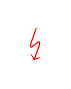
\begin{tikzpicture}[scale=0.2]
			\draw[rounded corners=3pt, rotate=10, red,
					->] (0.75,2)--(0,0.66)--(1,1.33)--(0.25,0);
		\end{tikzpicture}}
\newcommand{\indirektfelteves}
		{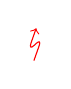
\begin{tikzpicture}[scale=0.2]
			\draw[rounded corners=3pt, rotate=10, red,
					<-] (0.75,2)--(0,0.66)--(1,1.33)--(0.25,0);
		\end{tikzpicture}}

\newcommand{\pecset}[2]{\begin{tikzpicture}[remember picture,overlay]
\node [ draw=red,
        rectangle,
        rounded corners=5mm,
        inner sep=1mm,
        ultra thick,
        fill=white,
        fill opacity=.8,
        rotate=30,
        scale=#1,
        text opacity=0.7]
        at (current page.center)
        {#2};
\end{tikzpicture}}

%\felirat{inner sep}{rounded corners}{scale}{x}{y}{text}
\newcommand{\felirat}[7][]{\begin{tikzpicture}[remember picture,overlay]
\node [draw=DeepSkyBlue3, rectangle, rounded corners=#3 mm, inner sep=#2mm, ultra thick, fill=white, fill opacity=.8, scale=#4, text opacity=1,#1]
at ([xshift=#5 cm, yshift=#6 cm]current page.center) {#7};
\end{tikzpicture}}

\newcommand{\hazi}[6]{\begin{tikzpicture}[remember picture,overlay]
\node [ draw=Coral1,
        rectangle,
        rounded corners=#2 mm,
        inner sep=#1mm,
        ultra thick,
        fill=white,
        fill opacity=.8,
        rotate=0,
        scale=#3,
        text opacity=1]
        at ([xshift=#4 cm, yshift=#5 cm]current page.center)
        {#6};
\end{tikzpicture}}


% Emphasizing:
\definecolor{barna}{rgb}{0.5,0.2,0.1}
\newcommand{\bemph}[1] {{\color{DeepSkyBlue3}{#1}}}
\newcommand{\kemph}[1] {{\color{blue}{#1}}}
\newcommand{\cemph}[1]{\textcolor{red}{#1}}
\newcommand{\zemph}[1] {{\color{Green2}{#1}}}
\newcommand{\yemph}[1] {{\color{Orange1}{#1}}}
\renewcommand{\emph}[1]{\textbf{#1}}

\newcommand{\FD}{\mathbf F}
\newcommand{\FB}{\mathbf G}
\newcommand{\PD}{\mathbf P}
\newcommand{\PB}{\mathbf H}

\newcommand{\FDDot}{\underline{\mathbf F}}
\newcommand{\FBDot}{\underline{\mathbf G}}
\newcommand{\PDDot}{\underline{\mathbf P}}
\newcommand{\PBDot}{\underline{\mathbf H}}


% i dont know whats this
\newcommand{\matbuborek}[1]{%
\begin{tikzpicture}
\node[draw=black, rounded corners=2pt, rectangle, inner sep=1mm] at (0,0){$#1$};
\end{tikzpicture}}


\newcommand{\dzsa}[1]{\textsc{\underline{#1}}:}

% modal operators:
 \newcommand{\diamondmeret}{.18}
 \newcommand{\boxmeret}{4*\diamondmeret/5}


 \newcommand{\mland} [1][.1]{\hspace{#1cm}\textup{and}\hspace{#1cm}}
 \newcommand{\mlthen}[1][.1]{\hspace{#1cm}\Rightarrow\hspace{#1cm}}
 \newcommand{\mlnot} [1][.1]{\hspace{#1cm}\textup{not }}
 \newcommand{\mlor}  [1][.1]{\hspace{#1cm}\textup{or}\hspace{#1cm}}
 \newcommand{\mliff} [1][.1]{\hspace{#1cm}\mliff\hspace{#1cm}}
 \newcommand{\vonal} [1][.2]{\hspace{#1cm} | \hspace{#1cm}}
 \newcommand{\mlwhere} [1][.2]{\hspace{#1cm}\textup{where}\hspace{#1cm}}
 \newcommand{\lrule}[3][c]{\begin{array}{#1} #2  \\  \hline #3 \end{array}}
 \newcommand{\dlrule}[3][c]{\begin{array}{#1} #2  \\  \hline\hline #3 \end{array}}
 \newcommand{\dual}{\delta}
\newcommand{\Dajmond}{\lozenge}
\newcommand{\Boksz}{\square}
\newcommand{\felDajmond}{\blacklozenge}
\newcommand{\felBoksz}{\blacksquare}
\newcommand{\Pmodels}{\mathrel{\models \hspace{-1.8ex} \raisebox{1.1ex}{\scalebox{.5}{$\mathrm{\bemph{P}}$}} }\,}
\newcommand{\Omodels}{\mathrel{\models \hspace{-1.8ex} \raisebox{1.1ex}{\scalebox{.5}{$\mathrm{\bemph{O}}$}} }\,}
\newcommand{\Kmodels}{\mathrel{\models \hspace{-1.8ex} \raisebox{1.1ex}{\scalebox{.5}{$\mathrm{\bemph{K}}$}} }\,}
\newcommand{\Bmodels}{\mathrel{\models \hspace{-1.8ex} \raisebox{1.1ex}{\scalebox{.5}{$\mathrm{\bemph{B}}$}} }\,}
\newcommand{\felle}	
	{\,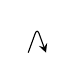
\begin{tikzpicture}
		\pgfmathsetmacro{\szog}{70}
		\pgfmathsetmacro{\hossz}{0.33}
	\draw[->,>=stealth,rounded corners=2pt] (0,0)	--(\szog:\hossz cm)
								--([shift=(-\szog :\hossz cm)]\szog:\hossz cm);	
	\end{tikzpicture}\,}
\newcommand{\lefel}
	{\, 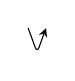
\begin{tikzpicture}
		\pgfmathsetmacro{\szog}{70}
		\pgfmathsetmacro{\hossz}{0.33}
		\draw[->,>=stealth,rounded corners=2pt] (0,0)	--(-\szog:\hossz cm)
								--([shift=(\szog :\hossz cm)]-\szog:\hossz cm);
	\end{tikzpicture}\, }
\newcommand{\enn}
{\mathbf{N}}
\newcommand{\nne}
{\reflectbox{$\mathbf{N}$}}

\newcommand{\mono}{\rightarrowtail}
\newcommand{\epi}{\twoheadrightarrow}
\newcommand{\iso}{\rightarrowtail \!\!\!\!\! \rightarrow}

 \newcommand{\defegy}[1][.1]{\hspace{#1cm}\overset{\textup{\tiny def}}{=}\hspace{#1cm}}
 \newcommand{\defpont}[1][.1]{\hspace{#1cm}\overset{\textup{\tiny def}}{:}\hspace{#1cm}}
 \newcommand{\defekv}[1][.1]{\hspace{#1cm}\overset{\textup{\tiny def}}{ \Leftrightarrow }\hspace{#1cm}}
 \newcommand{\lthen}{\rightarrow}
 \newcommand{\liff}{\leftrightarrow}
 \newcommand{\lminus}{-}
 \newcommand{\lsup}{\mbox{$\mathop{\sim}$}}
 \newcommand{\colnot}{\mbox{$\mathop{\sim}$}}
 \newcommand{\forallin}[2]{(\forall #1 \in #2)}
 \newcommand{\existsin}[2]{(\exists #1 \in #2)}
 \newcommand{\nexistsin}[2]{(\nexists #1 \in #2)}
 \newcommand{\forallp}[1]{(\forall #1)}
 \newcommand{\existsp}[1]{(\exists #1)}
 \newcommand{\forallR}[2]{(\forall #1 \reflectbox{$R$} #2)}
 \newcommand{\existsR}[2]{(\exists #1 \reflectbox{$R$} #2)}
\newcommand{\magyarazat}[2]{\overset{\substack{\textup{#2}\\ \downarrow}}{#1}}
\newcommand{\magyi}[1]{\textup{\bemph{\tiny #1}}}


\newcommand{\bintension}[2][]{{{[}\!{[}} {#2}{{]}\!{]}}^{\mathcal{#1}}}
\newcommand{\wintension}[3][]{{[}\hspace{-.46mm}{[} {#3}{]}\hspace{-.46mm}{]}^{\mathfrak{#1}}_{#2}}
\newcommand{\canintension}[2][]{{[}\hspace{-.46mm}{[} {#2}{]}\hspace{-.46mm}{]}_{\mathrm{#1}}}
\newcommand{\jelentes}[2]{{{[}\!{[}} {#1}{{]}\!{]}}^{{#2}}}
\newcommand{\intension}[2][]{{[}\hspace{-.46mm}{[} {#2}{]}\hspace{-.46mm}{]}^{\mathfrak{#1}}}
\newcommand{\Kintension}[2][]{|\!| {#2} |\!|^{\mathcal{#1}}}
\newcommand{\theory}[2][]{\mathrm{th}_{\mathfrak{#1}}(#2)}
\newcommand{\seenby}{\reflectbox {$R$}}
\newcommand{\derives}[1][]{\vdash_{\mathrm{#1}}}
\newcommand{\ugyanaz}[1]{\mathrel{\overset{#1}{\equiv}}}


\newcommand{\harmasosztas}[6]{

\begin{minipage}{#1\textwidth}%
#4%
\end{minipage}%
\begin{minipage}{#2\textwidth}%
#5%
\end{minipage}%
\begin{minipage}{#3\textwidth}%
#6%
\end{minipage}

}


\newcommand{\felkor}[8]{%
\begin{scope}[draw=#5,very thick,fill opacity=.15,draw opacity=.5,text opacity=1]
\draw[fill=#5]
([shift=(#3:#2)]#1) arc (#3:180+#3:#2) -- cycle;
\node at ([shift=(#7*180+#3:#2),shift=(-#7*90+135+#3:0.5*#6)]#1){#8};
\clip ([shift=(#3:#2)]#1) arc (#3:180+#3:#2);
 \draw[fill=#5] ([shift=(#7*180+#3:#2)]#1) circle (#6);
\end{scope}
}
\newcommand{\felkorvonal}[2]{
\draw[rounded corners=0] (180+#1:.25*#2 cm) arc (180+#1:360+#1:.25*#2 cm)--cycle;
}


\newcommand{\BoxTemplate}[1]{{#1} \mathop{\Box\hspace{-1.35ex} \raisebox{.5ex}{\scalebox{.5}{$\lthen$}}}}
\newcommand{\DiamondTemplate}[1]{#1\hspace{-.2ex} \mathop{\Diamond\hspace{-1.35ex} \raisebox{.4ex}{\scalebox{.5}{$\land$}}}\,}

%%%%%%%%%%%%%%%%%%%%%%%%%%%%%%%%%%%%%%%%%%%%%%%%%%%%%%
\newenvironment{tomb}[2][.1]{\arraycolsep=#1cm\begin{array}{#2}}{\end{array}}
\beamertemplatenavigationsymbolsempty


\author{Attila Moln\'ar}
\date{2014. March 21.}
\title{Axiomatization of Kripkean FOML}
\institute{ELTE}
\begin{document}
\footnotesize


\begin{frame}
\centering
\textsc{\Large Relativistic Temporal Logic \\[1em] Ways of Indeterminism}

\bigskip

{ \small Attila Moln\'ar

    \textit{E\"otv\"os Lor\'and University}}

 \begin{figure}

\includegraphics[scale=.3]{elte_cimer.png}
 \end{figure}

	\today
\end{frame}

%%%%%%%%%%%%%%%%%%%%%%%%%%%%%%%%%%%%%%%%%%%% NEXT SLIDE %%%%%%%%%%%%%%%%%%%%%%%%%%%%%%%%%%%%%%%%%%%%%

\szakasz[Trees]{Tree of Time}

\begin{frame}
	\frametitle{Indeterminist frames}
\footnotesize

\bigskip

\begin{minipage}{.7\textwidth}
Consider the tree on the right.
Let $p$ represent the sentence ``There is a sea battle''.
Suppose that $w$ is today, and $w_1$ and $w_2$ are the two possible tomorrows.
We have that $w \models \FD p \land \FD \lnot p$, therefore, %what does $\FD p$ mean?
\end{minipage}


\felirat{1.5}{1}{1}{4}{2.5}{
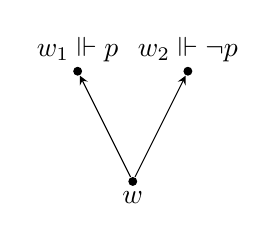
\begin{tikzpicture}[world/.style={inner sep=.4mm, fill=black, circle},>=stealth, scale=.7]
\node[world] (v1) at (0,-2) {};
\node[world] (v2) at (-1,0) {};
\node[world] (v3) at (1,0) {};
\node[anchor=south] at (v2) {$w_1\Vdash p$};
\node[anchor=south] at (v3) {$w_2\Vdash \lnot p$};
\node[anchor=north] at (v1) {$w$};
\draw[->]  (v1) edge (v2);
\draw[->]  (v1) edge (v3);
\end{tikzpicture}
}


\pause %%%%%%%%%%%%%%%%%% --- PAUSE --- %%%%%%%%%%%%%%%%%%

\bigskip

\begin{itemize}
\item Since $\FD p$ means ``It \emph{will} be true (tomorrow) that $p$'', in $w$ it is true that
\\ \begin{center}\scriptsize ``It will be true (tomorrow) that there is sea battle and \\ It will be true (tomorrow) that there is no see battle''.\end{center}
\pause %%%%%%%%%%%%%%%%%% --- PAUSE --- %%%%%%%%%%%%%%%%%%
\item Since $\FD p$ means ``\emph{In the future (tomorrow), it would be possible} that $p$'', in $w$ it is true that
\\ \begin{center}\scriptsize  ``In the future (tomorrow), it would be possible that there is a sea battle and \\In the future (tomorrow), it would be possible that there is no see battle''.\end{center}
\end{itemize}

\pause %%%%%%%%%%%%%%%%%% --- PAUSE --- %%%%%%%%%%%%%%%%%%

\vfill

So trees are appropriate drawings but somehow not ``will'' is the appropriate word for $\FD$. But then what is the meaning of ``will'' here?.

\end{frame}

%%%%%%%%%%%%%%%%%%%%%%%%%%%%%%%%%%%%%%%%%%%% NEXT SLIDE %%%%%%%%%%%%%%%%%%%%%%%%%%%%%%%%%%%%%%%%%%%%%

\begin{frame}
	\frametitle{Histories}
\footnotesize

Consider the trees as a \emph{bundle} of linear frames, that are called \emph{histories} in that context.

\[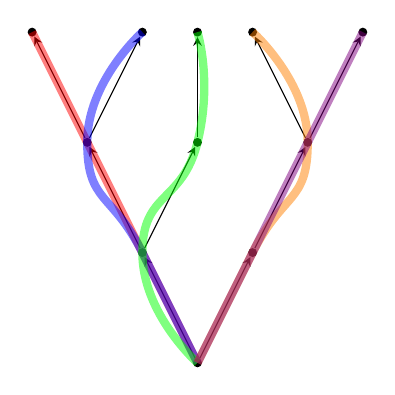
\begin{tikzpicture}[world/.style={inner sep=.4mm, fill=black, circle},>=stealth, scale=.7]
\node[world] (v1) at (0,-2) {};
\node[world] (v2) at (-1,0) {};
\node[world] (v3) at (1,0) {};
\node[world] (v4) at (-2,2) {};
\node[world] (v5) at (0,2) {};
\node[world] (v6) at (-3,4) {};
\node[world] (v9) at (2,2) {};
\node[world] (v10) at (1,4) {};
\node[world] (v11) at (3,4) {};
\node[world] (v8) at (0,4) {};
\node[world] (v7) at (-1,4) {};
\draw[->]  (v1) edge (v2);
\draw[->]  (v1) edge (v3);
\draw[->]  (v2) edge (v4);
\draw[->]  (v2) edge (v5);
\draw[->]  (v4) edge (v6);
\draw[->]  (v4) edge (v7);
\draw[->]  (v5) edge (v8);
\draw[->]  (v3) edge (v9);
\draw[->]  (v9) edge (v10);
\draw[->]  (v9) edge (v11);
\begin{scope}[line width=3, opacity=.5]
\pause %%%%%%%%%%%%%%%%%% --- PAUSE --- %%%%%%%%%%%%%%%%%%
\draw[red]    plot[smooth, tension=1] coordinates {(v1) (v2) (v4) (v6)};
\pause %%%%%%%%%%%%%%%%%% --- PAUSE --- %%%%%%%%%%%%%%%%%%
\draw[blue]   plot[smooth, tension=1] coordinates {(v1) (v2) (v4) (v7)};
\pause %%%%%%%%%%%%%%%%%% --- PAUSE --- %%%%%%%%%%%%%%%%%%
\draw[green]  plot[smooth, tension=1] coordinates {(v1) (v2) (v5) (v8)};
\pause %%%%%%%%%%%%%%%%%% --- PAUSE --- %%%%%%%%%%%%%%%%%%
\draw[orange] plot[smooth, tension=1] coordinates {(v1) (v3) (v9) (v10)};
\pause %%%%%%%%%%%%%%%%%% --- PAUSE --- %%%%%%%%%%%%%%%%%%
\draw[violet] plot[smooth, tension=1] coordinates {(v1) (v3) (v9) (v11)};
\end{scope}
\end{tikzpicture}\]
\end{frame}

%%%%%%%%%%%%%%%%%%%%%%%%%%%%%%%%%%%%%%%%%%%% NEXT SLIDE %%%%%%%%%%%%%%%%%%%%%%%%%%%%%%%%%%%%%%%%%%%%%

\begin{frame}
	\frametitle{Histories}
\footnotesize

Let $\mathfrak F= (W, <)$ be a tree.
\bigskip

\dzsa{Definition} A \emph{history} $h$ is a maximally linear subset of $W$, i.e.,

\begin{itemize}
\item linear: $\forallin {w,v}h \; w<v \lor w=v \lor w>v $.
\item there is no proper linear extension of it:
\[ \forallp {h'\supseteq h} \big[ h' \textup{ is linear } \lthen h'\subseteq h.\big]\]
\end{itemize}

$h\overset w \sim h'$ will mean that histories $h$ and $h'$ share the same past until $w$. Since we are working with trees, this can be formalized simply by %\[ h\overset w \sim h' \defekv w\in h\cap h' \textup{ and } \forallp {v<w} (v\in h \iff v\in h') \]
%Note that this definition is the same as
\[ h\overset w \sim h' \defekv w\in h\cap h' \]


The set of all histories of a frame will be denoted by $\mathrm H (\mathfrak F)$:
\[\mathrm H (\mathfrak F) \defegy \{ h\subseteq W : \textup{ $h$ is maximally linear}\}\]

\pause %%%%%%%%%%%%%%%%%% --- PAUSE --- %%%%%%%%%%%%%%%%%%

\hazi{2}{1}{.7}{0}{-4}{\begin{tabular}{l} show that $\overset w\sim$ is an equivalence relation.\end{tabular}}
\end{frame}

%%%%%%%%%%%%%%%%%%%%%%%%%%%%%%%%%%%%%%%%%%%% NEXT SLIDE %%%%%%%%%%%%%%%%%%%%%%%%%%%%%%%%%%%%%%%%%%%%%

\begin{frame}
	\frametitle{\large Indeterminist interpretations of the tense ``will''.}
\footnotesize

Read $\FD \varphi$ as ``it will be the case that $\varphi$''.

Is it plausible that

{\large
\[ (\FD \varphi \land \FD \psi)\, \lthen \, \big[ \FD(\varphi \land \FD \psi) \lor \FD(\varphi \land \psi) \lor \FD(\FD \varphi \land \psi)\big] \quad ? \]
}

{\scriptsize If $\varphi$ will be true and $\psi$ will be true, then at least one of the followings is true:
\begin{itemize}
\item $\varphi$ will be true, and after that $\psi$ will true.
\item $\psi$ will be true, and after that $\varphi$ will true.
\item $\varphi$ and $\psi$ will be true at the same time.
\end{itemize}}

\bigskip

\pause %%%%%%%%%%%%%%%%%% --- PAUSE --- %%%%%%%%%%%%%%%%%%

\textbf{Yes:} Ockhamist future

\bigskip

\pause %%%%%%%%%%%%%%%%%% --- PAUSE --- %%%%%%%%%%%%%%%%%%

\textbf{No:} Peircean future

\bigskip

All the other options are variations of these two.
\end{frame}

%%%%%%%%%%%%%%%%%%%%%%%%%%%%%%%%%%%%%%%%%%%% NEXT SLIDE %%%%%%%%%%%%%%%%%%%%%%%%%%%%%%%%%%%%%%%%%%%%%

\szakasz[Ockhamist]{Ockhamist future}

\begin{frame}
	\frametitle{Ockhamist future}
\footnotesize

{\scriptsize
\begin{center}
\begin{minipage}{.9\textwidth}
``Ockhamism'' [\dots] holds that it is meaningless to ask about the truth
value of ``a will happen'' at  $w$  without further specifications: the problem is
correctly expressed only if, in addition to $w$, one of its possible futures is specified.
``Will happen'' has to be understood as ``will happen in the specified future of $w$''.
\end{minipage}
\end{center}
\hfill \textsc{Zanardo 1996} (about \textsc{Prior 1967})
}

\begin{center}
\cemph{So the history is always a tacit parameter}
\end{center}

\pause %%%%%%%%%%%%%%%%%% --- PAUSE --- %%%%%%%%%%%%%%%%%%

\medskip

Indeterminism comes into the picture when we change the ``specified possible future'' (history) with an operator $\Diamond$.
\pause %%%%%%%%%%%%%%%%%% --- PAUSE --- %%%%%%%%%%%%%%%%%%
%\[ \mathfrak M, h, w \Omodels \varphi  \qquad \textup{\begin{minipage}{8cm}``in the model $\mathfrak M$, in the world $w$ of history $h$, $\varphi$ is true''\end{minipage}}\]
\\Let $\mathfrak M = (W, <, V)$ be a tree model.
%\pause %%%%%%%%%%%%%%%%%% --- PAUSE --- %%%%%%%%%%%%%%%%%%
\vspace{-1ex}\[\begin{tomb}[.15]{lcl}
%\textup{Ockhamist:}\\
   \mathfrak M , h, w \Omodels p &\defekv & w\in V(p)
\\ \mathfrak M , h, w \Omodels \lnot \varphi &\defekv & \textup{ it is not true that }\mathfrak M , h, w \Omodels \varphi
\\ \mathfrak M , h, w \Omodels \varphi \land \psi &\defekv & \mathfrak M , h, w \Omodels \varphi\textup{ and }\mathfrak M , h, w \Omodels \psi
\\ \mathfrak M , h, w \Omodels \PD \varphi &\defekv & \exists v \big( v<w \land \mathfrak M , h, v \Omodels \varphi\big)
\\ \mathfrak M , h, w \Omodels \FD \varphi &\defekv & \existsin v{\cemph{h}} \big( w<v \land \mathfrak M , h, v \Omodels \varphi\big)
\\ \mathfrak M , h, w \Omodels \Diamond \varphi &\defekv & \existsp {h'\overset w\sim h} \; \mathfrak M , h', w \Omodels \varphi
\end{tomb}\]
\end{frame}

%%%%%%%%%%%%%%%%%%%%%%%%%%%%%%%%%%%%%%%%%%%% NEXT SLIDE %%%%%%%%%%%%%%%%%%%%%%%%%%%%%%%%%%%%%%%%%%%%%
\begin{frame}
	\frametitle{Training}
\footnotesize
\[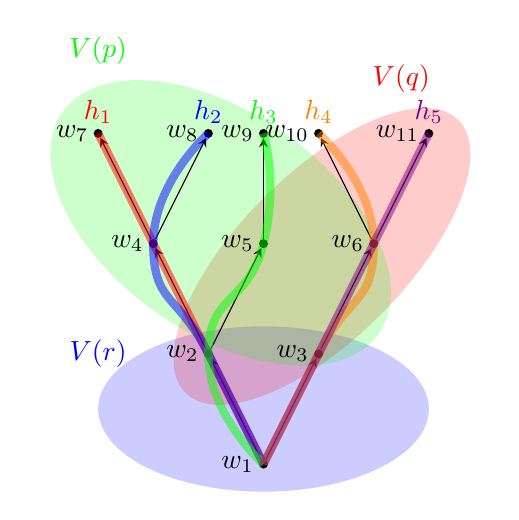
\begin{tikzpicture}[world/.style={inner sep=.4mm, fill=black, circle},>=stealth, scale=.7]

\begin{scope}[opacity=.2]
%\fill[red]  plot[smooth, tension=.7] coordinates {(-2,-1) (-0.5,-0.5) (1,1.5) (2.5,1.5) (4,4.5) (2.5,4.5) (-1,2) (-2.5,-0.5) (-2,-1)};
%\fill[green]  plot[smooth, tension=.7] coordinates {(-3.5,1.5) (3,1) (3.5,2.5) (0,3) (-1,4.5) (-4,4.5) (-3.5,1.5)};
\fill[blue]  (0,-1) ellipse (3 and 1.5);
\fill[red,rotate=45]  (2,0.5) ellipse (3.5 and 1.5);
\fill[green, rotate=-35]  (-2,1.5) ellipse (3.5 and 2);
\end{scope}
\node[world] (v1) at (0,-2) {};
\node[world] (v2) at (-1,0) {};
\node[world] (v3) at (1,0) {};
\node[world] (v4) at (-2,2) {};
\node[world] (v5) at (0,2) {};
\node[world] (v6) at (-3,4) {};
\node[world] (v9) at (2,2) {};
\node[world] (v10) at (1,4) {};
\node[world] (v11) at (3,4) {};
\node[world] (v8) at (0,4) {};
\node[world] (v7) at (-1,4) {};
\draw[->]  (v1) edge (v2);
\draw[->]  (v1) edge (v3);
\draw[->]  (v2) edge (v4);
\draw[->]  (v2) edge (v5);
\draw[->]  (v4) edge (v6);
\draw[->]  (v4) edge (v7);
\draw[->]  (v5) edge (v8);
\draw[->]  (v3) edge (v9);
\draw[->]  (v9) edge (v10);
\draw[->]  (v9) edge (v11);



\begin{scope}[line width=3, opacity=.5]
\draw[red]    plot[smooth, tension=1] coordinates {(v1) (v2) (v4) (v6)};
\draw[blue]   plot[smooth, tension=1] coordinates {(v1) (v2) (v4) (v7)};
\draw[green]  plot[smooth, tension=1] coordinates {(v1) (v2) (v5) (v8)};
\draw[orange] plot[smooth, tension=1] coordinates {(v1) (v3) (v9) (v10)};
\draw[violet] plot[smooth, tension=1] coordinates {(v1) (v3) (v9) (v11)};
\end{scope}
\begin{scope}[anchor=south]
\node[red] at (v6) {$h_1$};
\node[blue] at (v7) {$h_2$};
\node[green] at (v8) {$h_3$};
\node[orange] at (v10) {$h_4$};
\node[violet] at (v11) {$h_5$};
\end{scope}

\node[anchor=east] at (v4){$w_4$};
\node[anchor=east] at (v5){$w_5$};
\node[anchor=east] at (v9){$w_6$};
\node[anchor=east] at (v2){$w_2$};
\node[anchor=east] at (v3){$w_3$};
\node[anchor=east] at (v1){$w_1$};
\node[anchor=east] at (v6){$w_7$};
\node[anchor=east] at (v7){$w_8$};
\node[anchor=east] at (v8){$w_9$};
\node[anchor=east] at (v10){$w_{10}$};
\node[anchor=east] at (v11){$w_{11}$};

\node[green] at (-3,5.5) {$V(p)$};
\node[red] at (2.5,5) {$V(q)$};
\node[blue] at (-3,0) {$V(r)$};
\end{tikzpicture}\]

%\uncover<11->{
%$\mathfrak M, w \Pmodels \lnot \FD \lnot \varphi$ is true iff you can find a history of $w$ which evades $\lnot \varphi$, i.e., in which $\varphi$ is always true above $w$.}
\end{frame}

%%%%%%%%%%%%%%%%%%%%%%%%%%%%%%%%%%%%%%%%%%%% NEXT SLIDE %%%%%%%%%%%%%%%%%%%%%%%%%%%%%%%%%%%%%%%%%%%%%

\begin{frame}
	\frametitle{\large Ockhamist ``will''}
\footnotesize

{\large
\[ (\FD \varphi \land \FD \psi)\, \lthen \, \big[ \FD(\varphi \land \FD \psi) \lor \FD(\varphi \land \psi) \lor \FD(\FD \varphi \land \psi)\big] \quad ? \]
}

is valid because outside of $\varphi$ and $\psi$ there are no $\Diamond$-s, so once the meaning of $\varphi$ and $\psi$ is given, the meaning of the formula above is evaluated on a given history, which is a linear order of moments.


\end{frame}

%%%%%%%%%%%%%%%%%%%%%%%%%%%%%%%%%%%%%%%%%%%% NEXT SLIDE %%%%%%%%%%%%%%%%%%%%%%%%%%%%%%%%%%%%%%%%%%%%%

\szakasz[Peircean]{Peircean future}

\begin{frame}
	\frametitle{Peircean future}
\scriptsize

\begin{center}
\begin{minipage}{.9\textwidth}
From the Peircean point of view, [\dots] ``$\varphi$ will happen'' is short for ``$\varphi$ will happen, no
matter what possible future of $w$ is considered'', which is true just in case every
possible future of $w$ contains a moment at which $\varphi$ is true.
\end{minipage}
\end{center}
\hfill \textsc{Zanardo 1996} (about \textsc{Prior 1967})

\begin{center}
\cemph{So even if we use the histories to give the semantics of $\FD$, we do not relativize the truth of formulas to certain histories. Truth of a temporal statement is history-independent.}
\end{center}

\medskip

A set of worlds $X$ \emph{bars} $w$ iff every history containing $w$ goes through $X$:

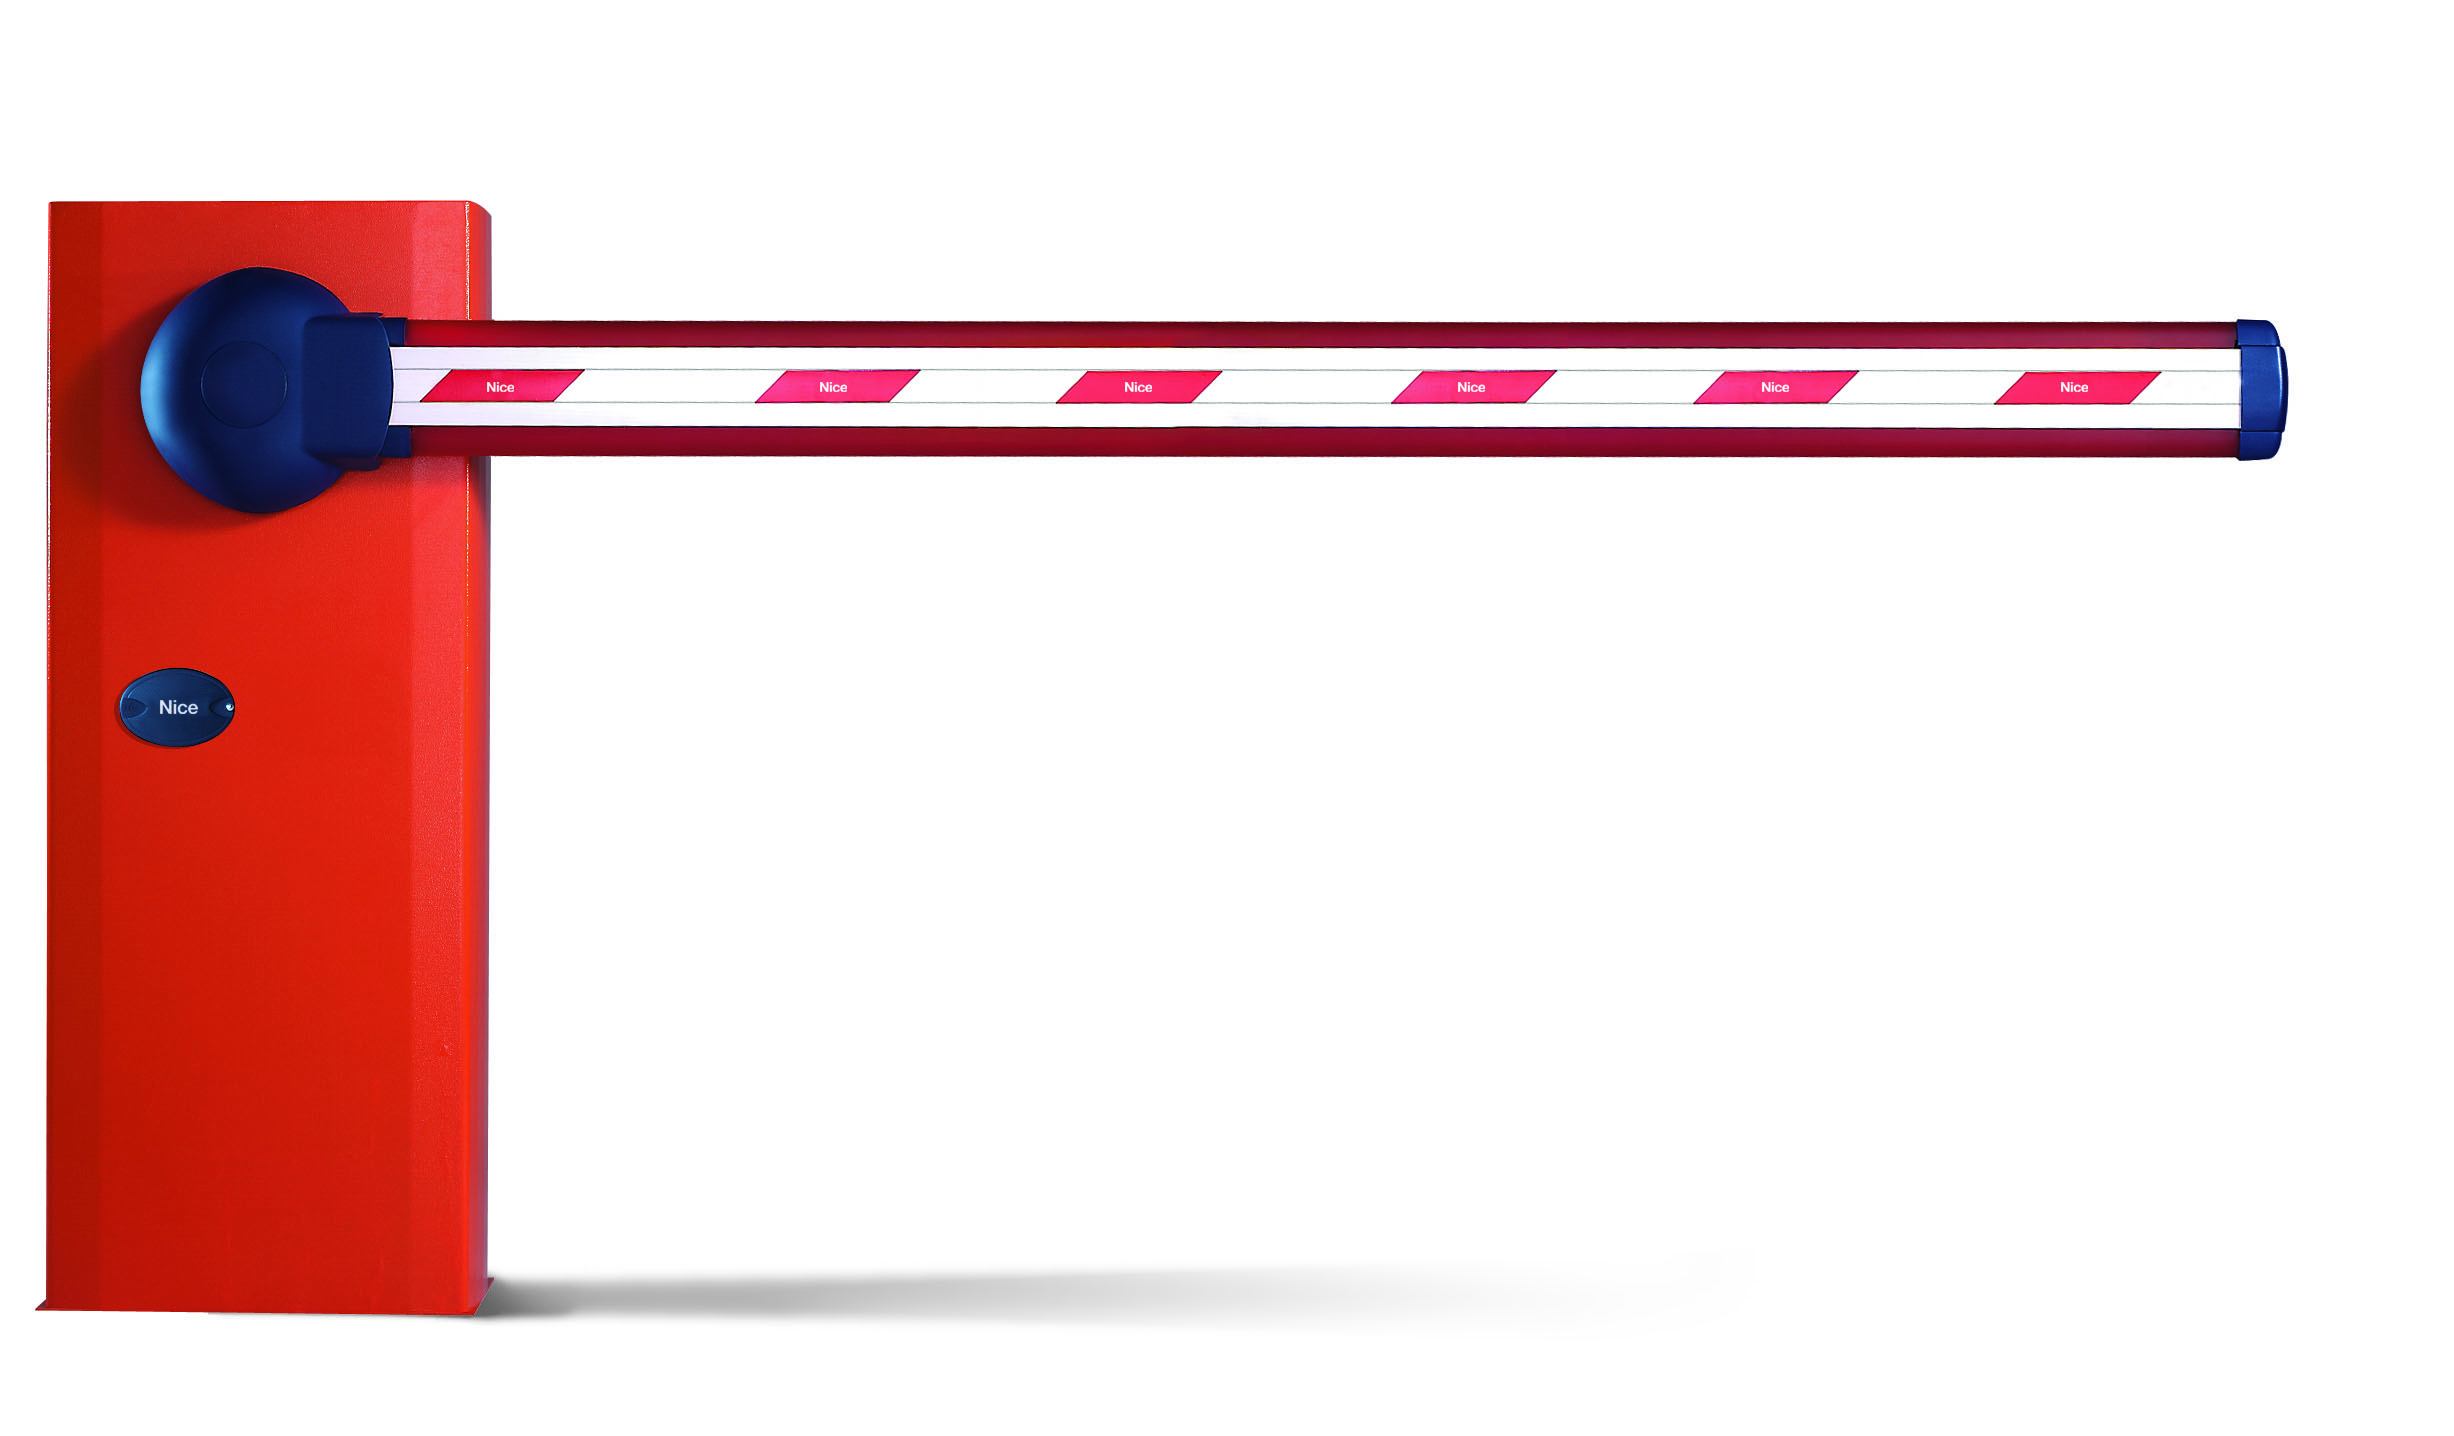
\includegraphics[scale=.02]{sorompo.jpg}
\qquad \raisebox{.3cm}{$\textup{$X$ bars $w$} \defekv \forallin h {\mathrm{H}({\mathfrak F})} (w\in h \lthen h\cap X\neq \varnothing) $}

Let $\mathfrak M = (W, <, V)$ be a tree model.
\\ $
\begin{tomb}[.15]{lcl}
\mathfrak M , w \Pmodels p &\defekv & w\in V(p)
\\ \mathfrak M , w \Pmodels \lnot \varphi &\defekv & \textup{ it is not true that }\mathfrak M , w \Pmodels \varphi
\\ \mathfrak M , w \Pmodels \varphi \land \psi &\defekv & \mathfrak M , w \Pmodels \varphi\textup{ and }\mathfrak M , w \Pmodels \psi
\\ \mathfrak M , w \Pmodels \PD \varphi &\defekv & \exists v \big( v<w \land \mathfrak M , v \Pmodels \varphi\big)
\\ \mathfrak M , w \Pmodels \FD \varphi &\defekv & %\forallin h{\mathrm{Hist}_{\mathfrak F}(w)} \existsin v{h} \big( w<v \land \mathfrak M , v \Pmodels \varphi\big)
%\\  &\Leftrightarrow &
\wintension[M]{\mathrm{\bemph P}}{\varphi} \textup{ bars } w
\end{tomb}
$

where $\wintension[M]{\mathrm{\bemph P}}{\varphi}\defegy \{w \, :\, \mathfrak M, w \Pmodels \varphi\}$, i.e, \\ the set of those worlds in which $\varphi$ is true.

\felirat{1.5}{1}{.6}{3.7}{-2.7}{
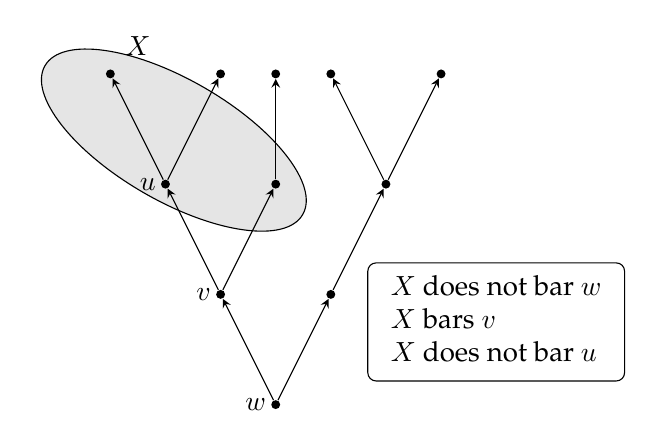
\begin{tikzpicture}[world/.style={inner sep=.4mm, fill=black, circle},>=stealth, scale=.7]
\filldraw[rotate=-30, fill opacity=.1]  (-3,1.5) ellipse (2.7 and 1.1);
\node at (-2.5,4.5) {$X$};
\node[world] (v1) at (0,-2) {};
\node[world] (v2) at (-1,0) {};
\node[world] (v3) at (1,0) {};
\node[world] (v4) at (-2,2) {};
\node[world] (v5) at (0,2) {};
\node[world] (v6) at (-3,4) {};
\node[world] (v9) at (2,2) {};
\node[world] (v10) at (1,4) {};
\node[world] (v11) at (3,4) {};
\node[world] (v8) at (0,4) {};
\node[world] (v7) at (-1,4) {};
\draw[->]  (v1) edge (v2);
\draw[->]  (v1) edge (v3);
\draw[->]  (v2) edge (v4);
\draw[->]  (v2) edge (v5);
\draw[->]  (v4) edge (v6);
\draw[->]  (v4) edge (v7);
\draw[->]  (v5) edge (v8);
\draw[->]  (v3) edge (v9);
\draw[->]  (v9) edge (v10);
\draw[->]  (v9) edge (v11);
\begin{scope}[anchor=east]
\node at (v1){$w$};
\node at (v2){$v$};
\node at (v4){$u$};
\end{scope}
\node[draw=black, rounded corners = 3] at (4,-0.5) {$\begin{array}{l}
X \textup{ does not bar }w
\\ X \textup{ bars }v
\\ X \textup{ does not bar }u
\end{array}$};
\end{tikzpicture}}
\end{frame}

%%%%%%%%%%%%%%%%%%%%%%%%%%%%%%% NEXT SLIDE %%%%%%%%%%%%%%%%%%%%%%%%%%%%%%%%%%%%%

\begin{frame}
	\frametitle{Training}
\footnotesize
\[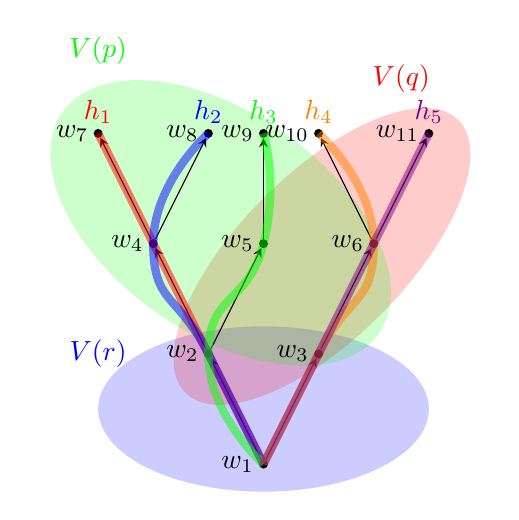
\begin{tikzpicture}[world/.style={inner sep=.4mm, fill=black, circle},>=stealth, scale=.7]

\begin{scope}[opacity=.2]
%\fill[red]  plot[smooth, tension=.7] coordinates {(-2,-1) (-0.5,-0.5) (1,1.5) (2.5,1.5) (4,4.5) (2.5,4.5) (-1,2) (-2.5,-0.5) (-2,-1)};
%\fill[green]  plot[smooth, tension=.7] coordinates {(-3.5,1.5) (3,1) (3.5,2.5) (0,3) (-1,4.5) (-4,4.5) (-3.5,1.5)};
\fill[blue]  (0,-1) ellipse (3 and 1.5);
\fill[red,rotate=45]  (2,0.5) ellipse (3.5 and 1.5);
\fill[green, rotate=-35]  (-2,1.5) ellipse (3.5 and 2);
\end{scope}
\node[world] (v1) at (0,-2) {};
\node[world] (v2) at (-1,0) {};
\node[world] (v3) at (1,0) {};
\node[world] (v4) at (-2,2) {};
\node[world] (v5) at (0,2) {};
\node[world] (v6) at (-3,4) {};
\node[world] (v9) at (2,2) {};
\node[world] (v10) at (1,4) {};
\node[world] (v11) at (3,4) {};
\node[world] (v8) at (0,4) {};
\node[world] (v7) at (-1,4) {};
\draw[->]  (v1) edge (v2);
\draw[->]  (v1) edge (v3);
\draw[->]  (v2) edge (v4);
\draw[->]  (v2) edge (v5);
\draw[->]  (v4) edge (v6);
\draw[->]  (v4) edge (v7);
\draw[->]  (v5) edge (v8);
\draw[->]  (v3) edge (v9);
\draw[->]  (v9) edge (v10);
\draw[->]  (v9) edge (v11);



\begin{scope}[line width=3, opacity=.5]
\draw[red]    plot[smooth, tension=1] coordinates {(v1) (v2) (v4) (v6)};
\draw[blue]   plot[smooth, tension=1] coordinates {(v1) (v2) (v4) (v7)};
\draw[green]  plot[smooth, tension=1] coordinates {(v1) (v2) (v5) (v8)};
\draw[orange] plot[smooth, tension=1] coordinates {(v1) (v3) (v9) (v10)};
\draw[violet] plot[smooth, tension=1] coordinates {(v1) (v3) (v9) (v11)};
\end{scope}
\begin{scope}[anchor=south]
\node[red] at (v6) {$h_1$};
\node[blue] at (v7) {$h_2$};
\node[green] at (v8) {$h_3$};
\node[orange] at (v10) {$h_4$};
\node[violet] at (v11) {$h_5$};
\end{scope}

\node[anchor=east] at (v4){$w_4$};
\node[anchor=east] at (v5){$w_5$};
\node[anchor=east] at (v9){$w_6$};
\node[anchor=east] at (v2){$w_2$};
\node[anchor=east] at (v3){$w_3$};
\node[anchor=east] at (v1){$w_1$};
\node[anchor=east] at (v6){$w_7$};
\node[anchor=east] at (v7){$w_8$};
\node[anchor=east] at (v8){$w_9$};
\node[anchor=east] at (v10){$w_{10}$};
\node[anchor=east] at (v11){$w_{11}$};

%\node[anchor=west] at (3.5,1) {$\begin{array}{c|c}
%\mathfrak M , h_1, w_4\Omodels \FB \textcolor{green}{p} & \pause %%%%%%%%%%%%%%%%%% --- PAUSE --- %%%%%%%%%%%%%%%%%% \textup{true}
%\\ \mathfrak M , h_1, w_2\Omodels \FB \textcolor{green}{p} & \pause %%%%%%%%%%%%%%%%%% --- PAUSE --- %%%%%%%%%%%%%%%%%%\textup{true}
%\\ \mathfrak M , h_1, w_2\Omodels \FB \lnot \textcolor{red}{q} & \pause %%%%%%%%%%%%%%%%%% --- PAUSE --- %%%%%%%%%%%%%%%%%%\textup{true}
%\\ \mathfrak M , ?, w_6\Omodels \FB \textcolor{red}{q} & \pause %%%%%%%%%%%%%%%%%% --- PAUSE --- %%%%%%%%%%%%%%%%%% h_5
%\\ \mathfrak M , w_6\Pmodels \FB \textcolor{red}{q} & \pause %%%%%%%%%%%%%%%%%% --- PAUSE --- %%%%%%%%%%%%%%%%%%\textup{false}
%\\ \mathfrak M , w_1 \Pmodels \FD \textcolor{green}{p} & \pause %%%%%%%%%%%%%%%%%% --- PAUSE --- %%%%%%%%%%%%%%%%%%\textup{true}
%\\ \mathfrak M , h_5, w_1 \Omodels \Box \FD \textcolor{blue}{r} & \pause %%%%%%%%%%%%%%%%%% --- PAUSE --- %%%%%%%%%%%%%%%%%%\textup{true}
%\\ \mathfrak M , h_5, w_1 \Omodels \Box \FB \textcolor{blue}{r} & \pause %%%%%%%%%%%%%%%%%% --- PAUSE --- %%%%%%%%%%%%%%%%%%\textup{false}
%\\ \mathfrak M , h_5, w_1 \Omodels \Diamond \FB \textcolor{blue}{r} & \pause %%%%%%%%%%%%%%%%%% --- PAUSE --- %%%%%%%%%%%%%%%%%%\textup{false}
%\\ \mathfrak M , w_1 \Pmodels \lnot \FD \lnot \textcolor{red}{q} & \pause %%%%%%%%%%%%%%%%%% --- PAUSE --- %%%%%%%%%%%%%%%%%%\textup{true}(!!)
%\end{array}$};

\node[green] at (-3,5.5) {$V(p)$};
\node[red] at (2.5,5) {$V(q)$};
\node[blue] at (-3,0) {$V(r)$};
\end{tikzpicture}\]

%\uncover<11->{
%$\mathfrak M, w \Pmodels \lnot \FD \lnot \varphi$ is true iff you can find a history of $w$ which evades $\lnot \varphi$, i.e., in which $\varphi$ is always true above $w$.}
\end{frame}

%%%%%%%%%%%%%%%%%%%%%%%%%%%%%%%%%%%%%%%%%%%% NEXT SLIDE %%%%%%%%%%%%%%%%%%%%%%%%%%%%%%%%%%%%%%%%%%%%%

\begin{frame}
	\frametitle{\large Peircean ``will''}
\footnotesize

{\large
\[ (\FD \varphi \land \FD \psi)\, \lthen \, \big[ \FD(\varphi \land \FD \psi) \lor \FD(\varphi \land \psi) \lor \FD(\FD \varphi \land \psi)\big] \quad ? \]
}

is invalid; let $\mathfrak M$ be the following ``twin lines''-model:
\[
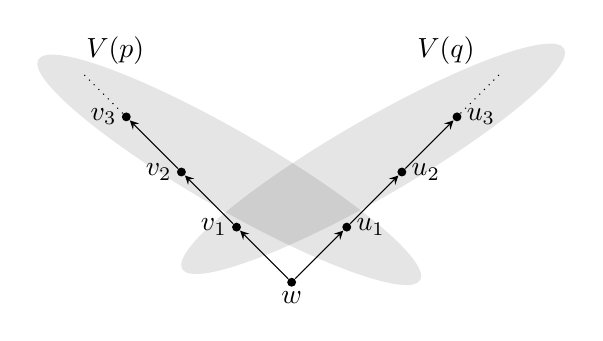
\begin{tikzpicture}[>=stealth, scale=.7,
world/.style={inner sep=.4mm, fill=black, circle},
intension/.style={fill=black, fill opacity=.1},
altrel/.style={->}]
\node [world] (v1) at (0,0) {};

\node [world] (v2) at (-1,1) {};
\node [world] (v3) at (1,1) {};
\node [world] (v4) at (-2,2) {};
\node [world] (v5) at (2,2) {};
\node [world] (v6) at (-3,3) {};
\node [world] (v7) at (3,3) {};
\node (v8) at (-4,4) {};
\node (v9) at (4,4) {};
\draw [altrel] (v1) edge (v2);
\draw [altrel] (v1) edge (v3);
\draw [altrel] (v2) edge (v4);
\draw [altrel] (v3) edge (v5);
\draw [altrel] (v4) edge (v6);
\draw [altrel] (v5) edge (v7);
\draw [dotted] (v6) edge (v8);
\draw [dotted] (v7) edge (v9);
\fill [intension, rotate=30] (2.4,1.2) ellipse (4 and .7);
\fill [intension, rotate=150] (2,-1.2) ellipse (4 and .7);
\node at (-3.2,4.2) {$V(p)$};
\node at (2.8,4.2) {$V(q)$};
\node[anchor=north] at (v1){$w$};
\node[anchor=east] at (v2){$v_1$};
\node[anchor=west] at (v3){$u_1$};
\node[anchor=east] at (v4){$v_2$};
\node[anchor=west] at (v5){$u_2$};
\node[anchor=east] at (v6){$v_3$};
\node[anchor=west] at (v7){$u_3$};
\end{tikzpicture}\]

\pause %%%%%%%%%%%%%%%%%% --- PAUSE --- %%%%%%%%%%%%%%%%%% \textup{true}
   $V(p)$ and $V(q)$ bars $w$, so $\mathfrak M, w \Pmodels \FD p \land \FD q$
\pause %%%%%%%%%%%%%%%%%% --- PAUSE --- %%%%%%%%%%%%%%%%%% \textup{true}
\\ $V(p)\cap V(q)= \varnothing$, and $\varnothing$ bars nothing, so $\mathfrak M, w \not\Pmodels \FD (p \land  q)$
\pause %%%%%%%%%%%%%%%%%% --- PAUSE --- %%%%%%%%%%%%%%%%%% \textup{true}
\\ $\wintension[M]{\bemph{P}}{\FD p} = \{w\}\cup \{ v_i \, : \, i\in \mathbb N \}$ \quad  $\wintension[M]{\bemph{P}}{\FD q} = \{w\}\cup \{ u_i \, : \, i\in \mathbb N \}$
\pause %%%%%%%%%%%%%%%%%% --- PAUSE --- %%%%%%%%%%%%%%%%%% \textup{true}
\\ $\wintension[M]{\bemph{P}}{\FD p}\cap V(q) = \{v_1\}$ \quad  $\wintension[M]{\bemph{P}}{\FD q}\cap V(p) = \{u_1\}$
\pause %%%%%%%%%%%%%%%%%% --- PAUSE --- %%%%%%%%%%%%%%%%%% \textup{true}
\\ But neither of these bars $w$, so $\mathfrak M, w \not\Pmodels \FD (\FD p \land  q)$ and $\mathfrak M, w \not\Pmodels \FD (p \land \FD  q)$

\end{frame}

%%%%%%%%%%%%%%%%%%%%%%%%%%%%%%% NEXT SLIDE %%%%%%%%%%%%%%%%%%%%%%%%%%%%%%%%%%%%%

\begin{frame}[t]
	\frametitle{``Always going to be \dots''}
Let $p$ represent the sentence ``The 3rd World War is on.''

How should we formalize the statement ``There won't be a 3rd World War.''?

\pause %%%%%%%%% PAUSE %%%%%%%%%%%%

\begin{itemize}
\item $\lnot \FD p $
\pause %%%%%%%%% PAUSE %%%%%%%%%%%%
\item $\FD \lnot p $
\end{itemize}

\pause %%%%%%%%% PAUSE %%%%%%%%%%%%
\hrule

\begin{itemize}
\item $\lnot \FD p $ says that $V(p)$ does not bar `us'. So there is an `escape' history in which the 3rd World War won't break out
\pause %%%%%%%%% PAUSE %%%%%%%%%%%%
\item $\FD \lnot p $ says that $W-V(p)$ bar `us'. So no matter what happens, there will be moments in the future when there is no 3rd World War.
\end{itemize}

\pause

None of the above is correct, because the first is speaking about \cemph{only some} `escape'-history, and the second talks about \cemph{only some} moments in the future in which there is no 3rd World war. The reason of course is that we interpret $\FD$ with a $\forall\exists$-way, and no matter how we negate it, the mixed nature of it will survive.

\bigskip

If we want to formalize the `won't-s, and ``always going to be''-s, we need the old history-independent strong future operator for that purpose:

\[\begin{tomb}[.15]{lcl}
\mathfrak M , w \Pmodels \FB \varphi &\defekv & \forall v \big( w<v \land \mathfrak M , v \Pmodels \varphi\big)
\end{tomb}\]

\end{frame}

\szakasz[Leibnizian]{Leibnizian}

\begin{frame}[t]
	\frametitle{Parallel histories}
\framesubtitle{Kamp frames instead of trees}
\footnotesize

\bigskip

\begin{minipage}{.7\textwidth}
Consider the tree on the right.
Let $p$ represent the sentence ``There is a sea battle''.
Suppose that $w$ \cemph{and $w'$ are}  today, and $w_1$ and $w_2$ are the two possible tomorrows.
\end{minipage}


\felirat{1.5}{1}{1}{4}{2.5}{
\only<1>{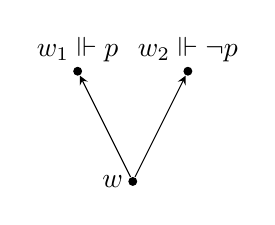
\begin{tikzpicture}[world/.style={inner sep=.4mm, fill=black, circle},>=stealth, scale=.7]
\node[world] (v1) at (0,-2) {};
\node[world] (v2) at (-1,0) {};
\node[world] (v3) at (1,0) {};
\node[anchor=south] at (v2) {$w_1\Vdash p$};
\node[anchor=south] at (v3) {$w_2\Vdash \lnot p$};
\node[anchor=east] at (v1) {$w$};
\draw[->]  (v1) edge (v2);
\draw[->]  (v1) edge (v3);
\end{tikzpicture}}
\only<2->{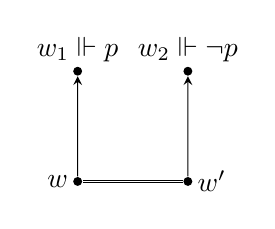
\begin{tikzpicture}[world/.style={inner sep=.4mm, fill=black, circle},>=stealth, scale=.7]
\node[world] (v1) at (-1,-2) {};
\node[world] (v2) at (-1,0) {};
\node[world] (v3) at (1,0) {};
\node(v1') [world] at (1,-2) {};
\node[anchor=south] at (v2) {$w_1\Vdash p$};
\node[anchor=south] at (v3) {$w_2\Vdash \lnot p$};
\node[anchor=east] at (v1) {$w$};
\node[anchor=west] at (v1') {$w'$};
\draw[->]  (v1) edge (v2);
\draw[->]  (v1') edge (v3);
\draw[double]  (v1') -- (v1);
\end{tikzpicture}}
}

\bigskip
\uncover<3->{
\[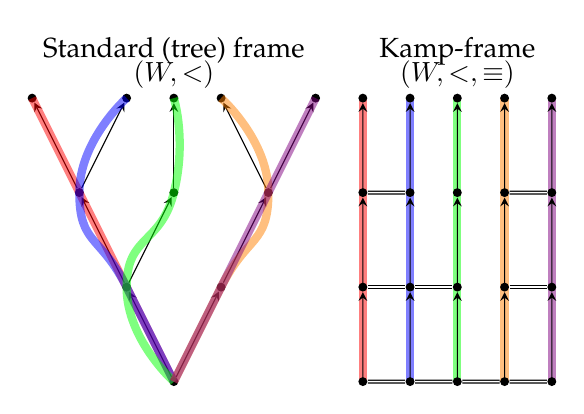
\begin{tikzpicture}[world/.style={inner sep=.4mm, fill=black, circle},>=stealth, scale=.6]



\node[world] (v1) at (0,-2) {};
\node[world] (v2) at (-1,0) {};
\node[world] (v3) at (1,0) {};
\node[world] (v4) at (-2,2) {};
\node[world] (v5) at (0,2) {};
\node[world] (v6) at (-3,4) {};
\node[world] (v9) at (2,2) {};
\node[world] (v10) at (1,4) {};
\node[world] (v11) at (3,4) {};
\node[world] (v8) at (0,4) {};
\node[world] (v7) at (-1,4) {};
\draw[->]  (v1) edge (v2);
\draw[->]  (v1) edge (v3);
\draw[->]  (v2) edge (v4);
\draw[->]  (v2) edge (v5);
\draw[->]  (v4) edge (v6);
\draw[->]  (v4) edge (v7);
\draw[->]  (v5) edge (v8);
\draw[->]  (v3) edge (v9);
\draw[->]  (v9) edge (v10);
\draw[->]  (v9) edge (v11);



\begin{scope}[line width=3, opacity=.5]
\draw[red]    plot[smooth, tension=1] coordinates {(v1) (v2) (v4) (v6)};
\draw[blue]   plot[smooth, tension=1] coordinates {(v1) (v2) (v4) (v7)};
\draw[green]  plot[smooth, tension=1] coordinates {(v1) (v2) (v5) (v8)};
\draw[orange] plot[smooth, tension=1] coordinates {(v1) (v3) (v9) (v10)};
\draw[violet] plot[smooth, tension=1] coordinates {(v1) (v3) (v9) (v11)};
\end{scope}

\foreach \x/\color in {1/red,2/blue,3/green,4/orange,5/violet}
{
\draw[line width=3, draw opacity=.5, draw=\color] (3+\x,-2)--(3+\x, 4);
\foreach \y in {0,2,4,6}{\node[world](w\x\y) at (3+\x, \y-2){};}
\foreach \y in {2,4,6}{\draw[->] (3+\x, \y-4) -- (w\x\y);}
}

\begin{scope}
\draw[double] (w10) -- (w20) ;
\draw[double] (w20) -- (w30) ;
\draw[double] (w30) -- (w40) ;
\draw[double] (w40) -- (w50) ;
%%%%%%%%%%%%
\draw[double] (w12) -- (w22) ;
\draw[double] (w22) -- (w32) ;
\draw[double] (w42) -- (w52) ;
%%%%%%%%%%%%
\draw[double] (w14) -- (w24) ;
%\draw (w24) -- (w34) ;
\draw[double] (w44) -- (w54) ;
\end{scope}

\node at (0,5) {Standard (tree) frame};
\node at (6,5) {Kamp-frame};

\node at (0,4.5) {$(W, <)$};
\node at (6,4.5) {$(W, <, \equiv)$};
\end{tikzpicture}
\]}


\end{frame}

%%%%%%%%%%%%%%%%%%%%%%%%%%%%%%%%%%%%%%%%%%%%%%%%%%%%%%%%%%%%%%%%%%%%%%%%%%%%%%%%%%%%%%%%%%%%%%%%%%%5

\begin{frame}
	\frametitle{Kamp-frames}

A Kamp-frame is a triplet $(W, <, \equiv)$ where
\begin{itemize}
\item $<$ is irreflexive, transitive and non-branching:
\begin{itemize}
\item $w\not < w$
\item $(w<v \land v<u )\lthen w<u$
\item $(w<v \land w<u) \lthen (v<u\lor v=u\lor v>u)$
\item $(w>v \land w>u) \lthen (v<u\lor v=u\lor v>u)$
\end{itemize}
\item $\equiv$ is reflexive, transitive and symmetric:
\begin{itemize}
\item $w\equiv w$
\item $(w\equiv v \land v\equiv u )\lthen w\equiv u$
\item $w\equiv v \lthen v\equiv w$
\end{itemize}
\item $x \equiv y \lthen x\not <y$ \hfill class irreflexivity
\item $(w \equiv v \land w'<w ) \lthen \existsp {v'<v} \;w'\equiv v'$  \hfill  ``sharing the same past''
\item $\forallp{w,v}\existsp{w'<w}\existsp {v'<v} \;w\equiv v$ \hfill class common root
\item $\forallp{w,v} (w \equiv v \land w\neq v) \existsp{w'>w}\forallp {v'>v} \;w'\not\equiv v'$ \\ \hfill maximality of histories
\end{itemize}

\felirat{1}{1}{.7}{4.5}{3}{
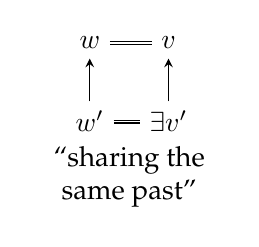
\begin{tikzpicture}[world/.style={inner sep=.4mm, fill=black, circle},>=stealth, scale=1]
\node (v1) at (0,0) {$w'$};
\node (v2) at (0,1) {$w$};
\node (v3) at (1,0) {$\exists v'$};
\node (v4) at (1,1) {$v$};
\draw[->]  (v1) -- (v2);
\draw[->]  (v3) -- (v4);
\draw[double]  (v1) -- (v3);
\draw[double]  (v2) -- (v4);
\node at (0.5,-0.7) {\begin{tabular}{c}``sharing the \\same past''\end{tabular}};
\end{tikzpicture}}
\felirat{1}{1}{.7}{4.5}{1.125}{
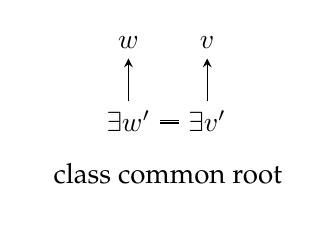
\begin{tikzpicture}[world/.style={inner sep=.4mm, fill=black, circle},>=stealth, scale=1]
\node (v1) at (0,0) {$\exists w'$};
\node (v2) at (0,1) {$w$};
\node (v3) at (1,0) {$\exists v'$};
\node (v4) at (1,1) {$v$};
\draw[->]  (v1) -- (v2);
\draw[->]  (v3) -- (v4);
\draw[double]  (v1) -- (v3);
%\draw[double]  (v2) -- (v4);
\node at (0.5,-0.7) {\begin{tabular}{c}class common root\end{tabular}};
\end{tikzpicture}}
\felirat{1}{1}{.7}{4.5}{-.75}{
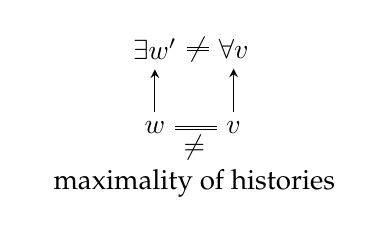
\begin{tikzpicture}[world/.style={inner sep=.4mm, fill=black, circle},>=stealth, scale=1]
\node at (0.5,-0.25) {$\neq$};
\node (v1) at (0,0) {$w$};
\node (v2) at (0,1) {$\exists w'$};
\node (v3) at (1,0) {$v$};
\draw[->]  (v1) -- (v2);
\draw[double]  (v1) -- (v3);
%\pause %%%%%%%%%%%%%%%%%% --- PAUSE --- %%%%%%%%%%%%%%%%%%
\node (v4) at (1,1) {$\forall v$};
\draw[double]  (v2) -- (v4);
\draw[->]  (v3) -- (v4);
\node at (0.5,-0.7) {\begin{tabular}{c}maximality of histories\end{tabular}};
\node at (0.5,1) {$\!\!\!\not$};
\end{tikzpicture}}
\pause

\hazi{1}{1}{.7}{-1}{-4.2}{\begin{minipage}{8cm}
Show that \begin{itemize}
\item class irreflexivity implies irreflexivity
\item maximality of histories implies class irreflexivity
\end{itemize}
\end{minipage}}

\end{frame}

%%%%%%%%%%%%%%%%%%%%%%%%%%%%%%%%%%%%%%%%%%%%%%%%%%%%%%%%%%%%%%%%%%%%%%%%%%%%%%%%%%%%%%%%%%%%%%%%%%%5
\begin{frame}
	\frametitle{Kamp-models}
Let $\mathfrak K=(W, <,\equiv)$ be a Kamp-frame. A Kamp-valuation is a $V:\mathrm{At}\to \wp W$ for which the following additional property holds:
\[ w\in V(p) \Rightarrow \forallp {v\equiv w}\; v\in V(p) \textup{ \qquad for all $p\in \mathrm{At}$} \]
a Kamp-frame $\mathfrak K=(W, <,\equiv)$ together with such a valuation $V$ is a Kamp-model $\mathfrak M_K=(\mathfrak K, V)$.


\[\begin{tomb}[.15]{lcl}
%\textup{Ockhamist:}\\
   \mathfrak M_K , w \Kmodels p &\defekv & w\in V(p)
\\ \mathfrak M_K , w \Kmodels \lnot \varphi &\defekv & \textup{it is not true that }\mathfrak M_K , w \Kmodels \varphi
\\ \mathfrak M_K , w \Kmodels \varphi \land \psi &\defekv & \mathfrak M_K , w \Kmodels \varphi\textup{ and }\mathfrak M_K , w \Kmodels \psi
\\ \mathfrak M_K , w \Kmodels \PD \varphi &\defekv & \existsp {v<w} \; \mathfrak M_K , v \Kmodels \varphi
\\ \mathfrak M_K , w \Kmodels \FD \varphi &\defekv & \existsp {v>w} \; \mathfrak M_K , v \Kmodels \varphi
\\ \mathfrak M_K , w \Kmodels \Diamond \varphi &\defekv & \existsp {v\equiv w} \; \mathfrak M_K, v \Kmodels \varphi
\end{tomb}\]
\end{frame}

%%%%%%%%%%%%%%%%%%%%%%%%%%%%%%%%%%%%%%%%%%%%%%%%%%%%%%%%%%%%%%%%%%%%%%%%%%%%%%%%%%%%%%%%%%%%%%%%%%%5

%%%%%%%%%%%%%%%%%%%%%%%%%%%%%%%%%%%%%%%%%%%%%%%%%%%%%%%%%%%%%%%%%%%%%%%%%%%%%%%%%%%%%%%%%%%%%%%%%%%5

\begin{frame}
	\frametitle{Kamp-frames}

\dzsa{Theorem} Every $\Kmodels$-valid formula is $\Omodels$-valid.

\bigskip
\pause
\dzsa{Proposition} There are $\Omodels$-valid formulas that are not $\Kmodels$-valid.
\pause
\bigskip

This was expected: $\Diamond$ in $\Kmodels$ quantifies over worlds, \\ \hfill but $\Omodels$ quantify over \cemph{sets of} worlds.

\bigskip

$\Diamond$ is interpreted with a 1st order quantification in $\Kmodels$
\\\hfill $\Diamond$ is interpreted with a 2nd order quantification in $\Omodels$

\pause
\bigskip

It is not impossible, however, to replace a 2nd order quantification with a 1st order one, but to do so, you have to be able to name all the sets with an individuum uniquely.

\pause

\hazi{2}{1}{.7}{0}{-4.2}{\begin{minipage}{11cm}
Show that every history \cemph{in a finite tree} is uniquely identifiable with a world.
\end{minipage}}


\end{frame}

%%%%%%%%%%%%%%%%%%%%%%%%%%%%%%%%%%%%%%%%%%%%%%%%%%%%%%%%%%%%%%%%%%%%%%%%%%%%%%%%%%%%%%%%%%%%%%%%%%%

\begin{frame}[t]
	\frametitle{Counterexample: Infinite binary trees}

\scriptsize
%Consider this grid of those points in the coordinatesystem, whose coordinates are positive integers.
\begin{minipage}{.55\textwidth}
    $W \defegy \{ w : w \textup{ is a route to a point}\}$
\\  $= \{ \langle w_1, \dots , w_n \rangle {:}\, n{\in} \omega, \forallp {i{\leq} n} w_i{\in} \{U,R\}\} $
\\[1em]  $w \sqsubseteq v \defekv \textup{$v$ is a continuation of $w$}$, i.e.,
\\       iff $\forallp {i\leq n} w_i= v_i $ where $n$ is the length of $w$.
\\[1em] Note that histories correspond to infinite routes!
\\[1em] Also note we can not name the histories by worlds (as was the case in the finite cases)! There are (infinitely) many infinite continutations of finite routes.
\\
\begin{minipage}{1.2cm}
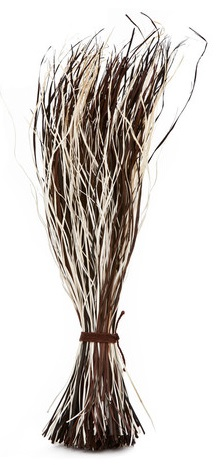
\includegraphics[scale=.15]{kepek/bundle.jpeg}
\end{minipage}
\begin{minipage}{4.5cm}
A set of histories $B\subseteq \mathrm{H}(\mathfrak F)$ is called a \textbf{bundle} iff \[ \bigcup B = W, \]
that is, for every $w\in W$ there is a history $h\in B$ s.t. $w\in h$.
\end{minipage}
\\ We can find a proper bundle, which is in fact can be named by worlds:
\[ \{ h\in \mathrm H(\mathfrak F) : \exists w \forallp {v>w} v=\langle w,U,\dots, U\rangle  \}\]
\end{minipage}
\begin{minipage}{.2\textwidth}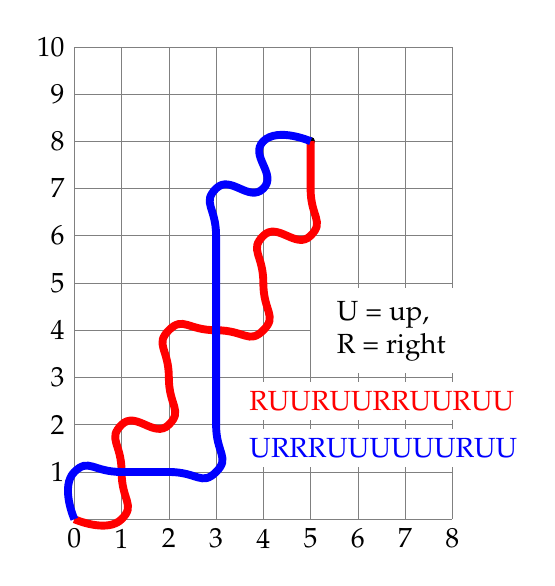
\begin{tikzpicture}[>=stealth, scale=.6,
world/.style={inner sep=.4mm, fill=black, circle},
intension/.style={fill=black, fill opacity=.1},
altrel/.style={->}]


%%%%%% SETTINGS %%%%%%%%%%

\pgfmathtruncatemacro{\gridwidth}{8}
\pgfmathtruncatemacro{\gridheight}{10}

%%%%%% RAJZ %%%%%%%%%%

\draw [help lines, step=1cm] (0,0) node (v1) {} grid (\gridwidth,\gridheight);

\foreach \i in {0, ..., \gridwidth}{\node [anchor=north] at (\i, 0) {\i};}
\foreach \i in {1, ..., \gridheight}{\node [anchor=east] at (0,\i) {\i};}

%\pause %%%%%%%%%%%% PAUSE %%%%%%%%%%%%%

\node [world] (v8) at (5,8) {};

%\pause %%%%%%%%%%%% PAUSE %%%%%%%%%%%%%


\begin{scope}[line width=1mm]
\draw[red]  plot[smooth, tension=1.1] coordinates {(v1) (1,0) (1,1) (1,2) (2,2) (2,3) (2,4) (3,4) (4,4) (4,5) (4,6) (5,6) (5,7) (v8)};
%\pause %%%%%%%%%%%% PAUSE %%%%%%%%%%%%%
\draw[blue]  plot[smooth, tension=1.1] coordinates {(v1) (0,1) (1,1) (2,1) (3,1) (3,2) (3,3) (3,4) (3,5) (3,6) (3,7) (4,7) (4,8) (v8)};
\end{scope}

%\pause %%%%%%%%%%%% PAUSE %%%%%%%%%%%%%


\begin{scope}[fill=white, anchor=west]
\node[fill=white, text=red] at (3.5,2.5) {RUURUURRUURUU};
\node[fill=white, text=blue] at (3.5,1.5) {URRRUUUUUURUU};
\node[fill=white, text=black] at (5,4) {\begin{tabular}{l}U = up,\\ R = right\end{tabular}};
\end{scope}

\end{tikzpicture}\end{minipage}
\end{frame}

%%%%%%%%%%%%%%%%%%%%%%%%%%%%%%%%%%%%%%%%%%% NEXT SLIDE %%%%%%%%%%%%%%%%%%%%%%%%%%%%%%%%%%%%%%%%%%%%%%%%%%%%%%%%5


\begin{frame}[t]
	\frametitle{Bundled trees}
\scriptsize

\dzsa{Definition} A bundled tree is a triplet $\mathfrak F_B=(W, <, B)$ where $(W,<)$ is a tree and $B\subseteq \mathrm{H}(W, <)$ is a bundle. A bundled model is a quadruple $(\mathfrak F_B, V)$ where $\mathfrak F_B$ is a bundled frame and $V: \mathrm{At}\to \wp W$ is a valuation.
\[\begin{tomb}[.15]{lcl}
%\textup{Ockhamist:}\\
   \mathfrak M , h, w \Bmodels p &\defekv & w\in V(p)
\\ \mathfrak M , h, w \Bmodels \lnot \varphi &\defekv & \textup{ it is not true that }\mathfrak M , h, w \Bmodels \varphi
\\ \mathfrak M , h, w \Bmodels \varphi \land \psi &\defekv & \mathfrak M , h, w \Bmodels \varphi\textup{ and }\mathfrak M , h, w \Bmodels \psi
\\ \mathfrak M , h, w \Bmodels \PD \varphi &\defekv & \exists v \big( v<w \land \mathfrak M , h, v \Bmodels \varphi\big)
\\ \mathfrak M , h, w \Bmodels \FD \varphi &\defekv & \existsin v{h} \big( w<v \land \mathfrak M , h, v \Bmodels \varphi\big)
\\ \mathfrak M , h, w \Bmodels \Diamond \varphi &\defekv & \existsp {h'\overset w\sim h} \;\big(\cemph{h\in B}\land \mathfrak M , h', w \Bmodels \varphi\big)
\end{tomb}\]

\dzsa{Proposition} $\Kmodels$-validity corresponds to $\Bmodels$-validity.

\bigskip

\dzsa{Quote} ``Belnap et al. have argued that it is implausible to assume that there could be some property which could >>justify treating some maximal chains as real possibilities and others as not<< (Belnap et al. 2001, p. 205)''
\\\hfill {\scriptsize Hirokazu Nishimura (1979) -- Stanford Enc.}


\end{frame}
%%%%%%%%%%%%%%%%%%%%%%%%%%%%%%%%%%%%%%%%%%%%%%%%%%%%%%%%%%%%%%%%%%%%%%%%%%
\begin{frame}[t]
	\frametitle{Defense of Bundled trees}
\scriptsize

Suppose we have discrete models (we are thinking in days instead of moments). Are these two sentences contradictory?
\begin{itemize}
\item ``Inevitably, if today there is life on earth, then either this is the last day (of life on earth), or the last day will come.''
\item ``At any possible day on which there is life on earth, it is possible that there will be life on earth the following day.''
\end{itemize}
\hfill {\scriptsize Hirokazu Nishimura (1979)-- Stanford Enc.}

Let $p$ be ``there is life on earth''. Let $h$ be some history (it does not matter actually)
\begin{itemize}
\item $\mathfrak M , h, w\models \Box (p \lthen \underline{\FD} \FB \lnot p)$
\item For all $v\in W$: $\mathfrak M, h, v \models p \lthen \Diamond \FD p$
\end{itemize}

\end{frame}
%%%%%%%%%%%%%%%%%%%%%%%%%%%%%%%%%%%%%%%%%%%%%%%%%%%%%%%%%%%%%%%%%%%%%%%%%%
\begin{frame}[t]
	\frametitle{Defense of Bundled trees}
\scriptsize

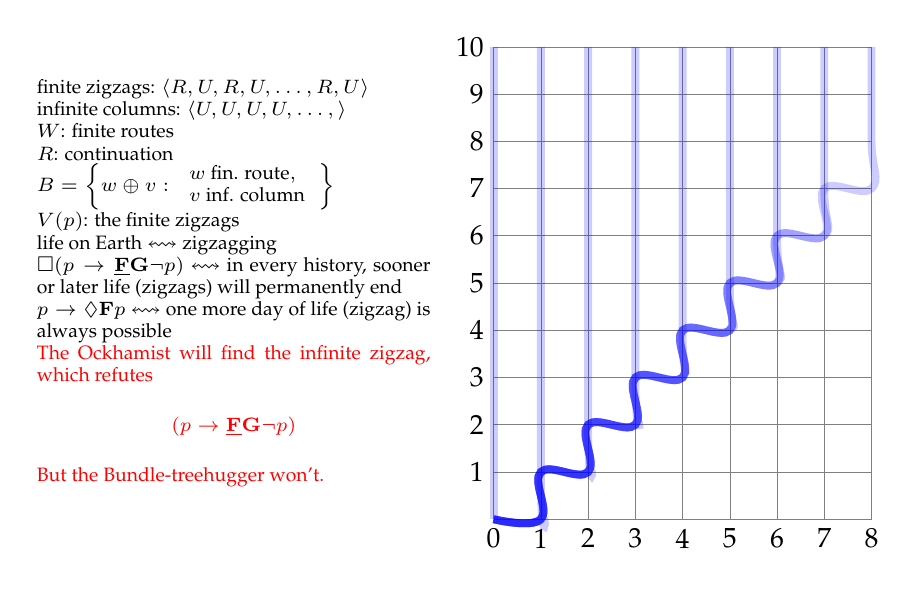
\begin{tikzpicture}[>=stealth, scale=.6,
world/.style={inner sep=.4mm, fill=black, circle},
intension/.style={fill=black, fill opacity=.1},
altrel/.style={->}]


%%%%%% SETTINGS %%%%%%%%%%

\pgfmathtruncatemacro{\gridwidth}{8}
\pgfmathtruncatemacro{\gridheight}{10}

%%%%%% RAJZ %%%%%%%%%%

\draw [help lines, step=1cm] (0,0) node (v1) {} grid (\gridwidth,\gridheight);

\foreach \i in {0, ..., \gridwidth}{\node [anchor=north] at (\i, 0) {\i};}
\foreach \i in {1, ..., \gridheight}{\node [anchor=east] at (0,\i) {\i};}

%\pause %%%%%%%%%%%% PAUSE %%%%%%%%%%%%%
%\pause %%%%%%%%%%%% PAUSE %%%%%%%%%%%%%


\begin{scope}[blue, line width=1mm, opacity=.2]
\draw  plot[smooth, tension=.7] coordinates {(v1)  (0,10) };
\draw  plot[smooth, tension=.7] coordinates {(v1) (1,0) (1,1) (1,10) };
\draw  plot[smooth, tension=.7] coordinates {(v1) (1,0) (1,1) (2,1) (2,2) (2,10) };
\draw  plot[smooth, tension=.7] coordinates {(v1) (1,0) (1,1) (2,1) (2,2) (3,2) (3,3) (3,10) };
\draw  plot[smooth, tension=.7] coordinates {(v1) (1,0) (1,1) (2,1) (2,2) (3,2) (3,3) (4,3) (4,4) (4,10) };
\draw  plot[smooth, tension=.7] coordinates {(v1) (1,0) (1,1) (2,1) (2,2) (3,2) (3,3) (4,3) (4,4) (5,4) (5,5) (5,10) };
\draw  plot[smooth, tension=.7] coordinates {(v1) (1,0) (1,1) (2,1) (2,2) (3,2) (3,3) (4,3) (4,4) (5,4) (5,5) (6, 5) (6,6) (6,10) };
\draw  plot[smooth, tension=.7] coordinates {(v1) (1,0) (1,1) (2,1) (2,2) (3,2) (3,3) (4,3) (4,4) (5,4) (5,5) (6, 5) (6,6) (7,6) (7,7) (7,10) };
\draw  plot[smooth, tension=.7] coordinates {(v1) (1,0) (1,1) (2,1) (2,2) (3,2) (3,3) (4,3) (4,4) (5,4) (5,5) (6, 5) (6,6) (7,6) (7,7) (8,7) (8,8) (8,10) };
\end{scope}


%\pause %%%%%%%%%%%% PAUSE %%%%%%%%%%%%%

\node at (-5.5,5) {
\begin{minipage}{5cm}\scriptsize
%    infinite zigzags: \\ \hfill $\langle R,U,R,U, \dots,\rangle$
 finite zigzags:   $\langle R,U,R,U, \dots, R,U\rangle$
\\ infinite columns:  $\langle U,U,U,U, \dots,\rangle$
\\ $W$: finite routes
\\ $R$: continuation
\\ $B= \left\{ w\oplus v: \begin{array}{l}w \textup{ fin. route}, \\ v \textup{ inf. column} \end{array}\right\}$
\\ $V(p)$: the finite zigzags
\\ life on Earth $\leftrightsquigarrow$ zigzagging
\\ $\Box (p\to \underline {\mathbf F} \mathbf G\lnot p)$ $\leftrightsquigarrow$ in every history, sooner or later life (zigzags) will permanently end
\\ $p\to \Diamond \mathbf F p$ $\leftrightsquigarrow$ one more day of life (zigzag) is always possible
\\ \textcolor{red}{The Ockhamist will find the infinite zigzag, which refutes
\[(p\to \underline {\mathbf F} \mathbf G\lnot p)\]
But the Bundle-treehugger won't.}
\end{minipage}};
\end{tikzpicture}

\end{frame}

\szakasz[Thomason]{Thomason}

\begin{frame}
	\frametitle{Truth value gaps for the \\ future contingents}
\footnotesize

\bigskip

\begin{minipage}{.7\textwidth}
Consider the tree on the right.
Let $p$ represent the sentence ``There is a sea battle''.
Suppose that $w$ is today, and $w_1$ and $w_2$ are the two possible tomorrows.
\end{minipage}


\felirat{1.5}{1}{1}{4}{2.5}{
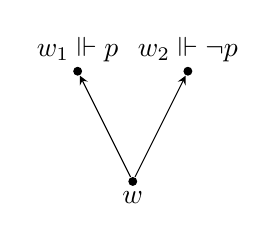
\begin{tikzpicture}[world/.style={inner sep=.4mm, fill=black, circle},>=stealth, scale=.7]
\node[world] (v1) at (0,-2) {};
\node[world] (v2) at (-1,0) {};
\node[world] (v3) at (1,0) {};
\node[anchor=south] at (v2) {$w_1\Vdash p$};
\node[anchor=south] at (v3) {$w_2\Vdash \lnot p$};
\node[anchor=north] at (v1) {$w$};
\draw[->]  (v1) edge (v2);
\draw[->]  (v1) edge (v3);
\end{tikzpicture}
}


\pause %%%%%%%%%%%%%%%%%% --- PAUSE --- %%%%%%%%%%%%%%%%%%

\bigskip

\begin{itemize}
\item $\FD p$ is true iff $V(p)$ bars the moment of utterance. (standard Peircean)
\pause %%%%%%%%%%%%%%%%%% --- PAUSE --- %%%%%%%%%%%%%%%%%%
\item $\FD p$ is false iff $V(\lnot p)$ bars the moment of utterance.
\pause %%%%%%%%%%%%%%%%%% --- PAUSE --- %%%%%%%%%%%%%%%%%%
\\[1em]{\scriptsize (Not Peircean at all!!! Falsehood of $\FD p$ correspond to the Peircean truth of $\FD \lnot p$, not to $\lnot \FD p$!! So from a Peircean point of view, falsehood is some kind of `inner negation'.)}
\end{itemize}

\pause %%%%%%%%%%%%%%%%%% --- PAUSE --- %%%%%%%%%%%%%%%%%%
\cemph{Partial semantics:} What if neither of them bar the moment of utterance?
\bigskip

\pause %%%%%%%%%%%%%%%%%% --- PAUSE --- %%%%%%%%%%%%%%%%%%
   Then $\FD p$ is \cemph{undefined} in the moment of utterance.
\pause %%%%%%%%%%%%%%%%%% --- PAUSE --- %%%%%%%%%%%%%%%%%%
Because these statements' truth values are not \cemph{settled} yet. Tomorrow they will be settled, but now they are not.

\felirat{1}{1}{.7}{3}{-4.25}{\begin{minipage}{7cm}Imre Ruzsa, the founder of this department, is a (the?) champion of partial modal semantics.\end{minipage}
}
\end{frame}

\begin{frame}
	\frametitle{Supervaluation}
\footnotesize

We will consider the word \cemph{undefined} as a 3rd truth value.

\felirat{1}{1}{.7}{4}{-3}{\begin{minipage}{5cm}Ruzsa was a hardcore classical logician as well: He did not acknowledged any formal system as a logic if it did not fulfilled the Law of (Non-)Contradiction and the Law of Excluded Middle. But how did he give an account about these 3-valued thing as a logic? These classical laws are fulfilled -- on those formulas where the interpretation is defined.\end{minipage}}

\pause %%%%%%%%%%%%%%%%%% --- PAUSE --- %%%%%%%%%%%%%%%%%%
\bigskip

\dzsa{Notational problem} we can not represent 3 value with our $\models$ sign, so we switch to the intension-notation:
\[\mathfrak M, w \models \varphi \leftrightsquigarrow \wintension[M]{w}{\varphi} = \textup{true} \]



\begin{minipage}{.7\textwidth}
\dzsa{Cheat} Instead of starting everything from the beginning, we can define truth via Ockhamist truth!

\begin{center}\scriptsize \dots Thomasonian truth \cemph{supervenes} on Ockhamist truth\dots\end{center}

\[ \wintension[M]{w}{\varphi} \defegy
\left\{ \begin{tomb}{ll}
   \mathrm T & \textup{ if } \forallp{h\ni w} \mathfrak M , h, w \Omodels \varphi
\\ \mathrm F & \textup{ if } \forallp{h\ni w} \mathfrak M , h, w \Omodels \lnot\varphi
\\ \mathrm U & \textup{ otherwise }
\end{tomb}\right. \]
\end{minipage}
\end{frame}

\begin{frame}
	\frametitle{Compositionality}
\footnotesize

Our cheat had a cost: the compositionality.

\bigskip

\dzsa{Definition} A meaning function $\wintension{w}{}$ is compositional iff the meaning $\wintension{w}{f(\varphi, \psi, \dots)}$ of a complex expression $f(\varphi, \psi, \dots)$ is determined by the meanings $\wintension{w}{\varphi}, \wintension{w}{\psi},\dots$ of the constituents $\varphi$, $\psi$, \dots

\hfill {\begin{minipage}{.6\textwidth} \scriptsize \begin{flushright}\bemph{That is a very general definition which is common in the Andréka--Németi--Madarász--Sain school}\end{flushright}\end{minipage}}

\pause %%%%%%%%%%%%%%%%%%% PAUSE %%%%%%%%%%%%%%%%%%%%%%%%

\bigskip

\begin{minipage}{.7\textwidth}
Remember to the sea battle model:
\[ \wintension{w}{\FD p} = \mathrm U, \qquad \wintension{w}{\FD \lnot p} = \mathrm U, \qquad \wintension{w}{\FD p \lor \FD \lnot p} = \mathrm T\]
But
\[ \wintension{w}{\FD p} = \mathrm U, \qquad \wintension{w}{\FD p} = \mathrm U, \qquad \wintension{w}{\FD p \lor \FD p} = \mathrm U\]

In non-compositional logics you have to ``look into'' the formula
\end{minipage}


\felirat{1.5}{1}{1}{4}{-2.5}{
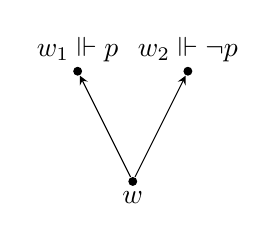
\begin{tikzpicture}[world/.style={inner sep=.4mm, fill=black, circle},>=stealth, scale=.7]
\node[world] (v1) at (0,-2) {};
\node[world] (v2) at (-1,0) {};
\node[world] (v3) at (1,0) {};
\node[anchor=south] at (v2) {$w_1\Vdash p$};
\node[anchor=south] at (v3) {$w_2\Vdash \lnot p$};
\node[anchor=north] at (v1) {$w$};
\draw[->]  (v1) edge (v2);
\draw[->]  (v1) edge (v3);
\end{tikzpicture}
}

\end{frame}

\szakasz[{\L}ukasiewitz?]{{\L}ukasiewitz?}
%%%%%%%%%%%%%%%%%%%%%%%%%%%  NEXT SLIDE %%%%%%%%%%%%%%%%%%%%%%%%%%%%%%%%%%%%%%%%%%%%%%%%%%%%%%55
\begin{frame}
	\frametitle{Modelling the undefined -- Kleene's logic(s)}
	\framesubtitle{Atoms and Negation}
Every atom is either true or false, given by the model's valuation $V$.
%We use the usual notion of tree models. (I.e., valuation are the same, so in every world, every $p$ and $q$ is either true or false.)
\[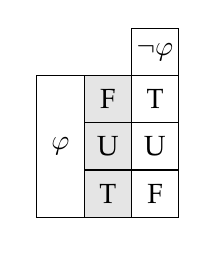
\begin{tikzpicture}[scale=.6]
\draw [step=1cm] (-1,-4) node (v1) {} grid (2,-1) node (v2) {};
\draw[fill=white]  (v1) rectangle (0,-1);
\draw  (v2) rectangle (1,0);
\draw[fill=black, opacity=.1]  (1,-1) rectangle (0,-4);
\node at (1.5,-0.5) {$\lnot \varphi$};
\node at (-0.5,-2.5) {$\varphi$};
% The gray area
%     gray row
\node at (0.5,-1.5) {F};
\node at (0.5,-2.5) {U};
\node at (0.5,-3.5) {T};
%     1st row
\node at (1.5,-1.5) {T};
%     2nd row
\node at (1.5,-2.5) {U};
%     3rd row
\node at (1.5,-3.5) {F};
\end{tikzpicture}
\]
\end{frame}
%%%%%%%%%%%%%%%%%%%%%%%%%%%  NEXT SLIDE %%%%%%%%%%%%%%%%%%%%%%%%%%%%%%%%%%%%%%%%%%%%%%%%%%%%%%55
\begin{frame}
	\frametitle{Modelling the undefined -- Kleene's logic(s)}
	\framesubtitle{Conjunction and Disjunction}
\footnotesize

\[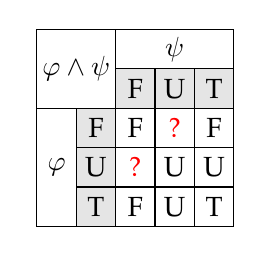
\begin{tikzpicture}[scale=.5]
\node at (0,0){};
\draw [step=1cm] (-1,-4) node (v1) {} grid (4,1);
\draw[fill=white]  (v1) rectangle (0,-1);
\draw[fill=white]  (-1,1) rectangle (1,-1) node (v2) {};
\draw[fill=white]  (1,1) rectangle (4,0);
\draw[fill=black, opacity=.1]  (v2) node (v3) {} rectangle (4,0);
\draw[fill=black, opacity=.1]  (v3) rectangle (0,-4);
\node at (0,0) {$\varphi\land \psi$};
\node at (-0.5,-2.5) {$\varphi$};
\node at (2.5,0.5) {$\psi$};
% The gray area
%     gray row
\node at (0.5,-1.5) {F};
\node at (0.5,-2.5) {U};
\node at (0.5,-3.5) {T};
%     gray column
\node at (1.5,-0.5) {F};
\node at (2.5,-0.5) {U};
\node at (3.5,-0.5) {T};
%     the white grid
%     1st row
\node at (1.5,-1.5) {F};
\node at (2.5,-1.5) {\cemph{?}};
\node at (3.5,-1.5) {F};
%     2nd row
\node at (1.5,-2.5) {\cemph{?}};
\node at (2.5,-2.5) {U};
\node at (3.5,-2.5) {U};
%     3rd row
\node at (1.5,-3.5) {F};
\node at (2.5,-3.5) {U};
\node at (3.5,-3.5) {T};
\end{tikzpicture}
\qquad %%%%%%%%%%%%%%%%%%%%%%%%%%%%%%%%%% KÉT KÉP KÖZTI SZÜNET %%%%%%%%%%%%%%%%%%%%%%%%%%%%%%%%%%%%%%%%%%%
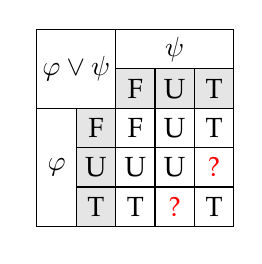
\begin{tikzpicture}[scale=.5]
\node at (0,0){};
\draw [step=1cm] (-1,-4) node (v1) {} grid (4,1);
\draw[fill=white]  (v1) rectangle (0,-1);
\draw[fill=white]  (-1,1) rectangle (1,-1) node (v2) {};
\draw[fill=white]  (1,1) rectangle (4,0);
\draw[fill=black, opacity=.1]  (v2) node (v3) {} rectangle (4,0);
\draw[fill=black, opacity=.1]  (v3) rectangle (0,-4);
\node at (0,0) {$\varphi\lor \psi$};
\node at (-0.5,-2.5) {$\varphi$};
\node at (2.5,0.5) {$\psi$};
% The gray area
%     gray row
\node at (0.5,-1.5) {F};
\node at (0.5,-2.5) {U};
\node at (0.5,-3.5) {T};
%     gray column
\node at (1.5,-0.5) {F};
\node at (2.5,-0.5) {U};
\node at (3.5,-0.5) {T};
%     the white grid
%     1st row
\node at (1.5,-1.5) {F};
\node at (2.5,-1.5) {U};
\node at (3.5,-1.5) {T};
%     2nd row
\node at (1.5,-2.5) {U};
\node at (2.5,-2.5) {U};
\node at (3.5,-2.5) {\cemph{?}};
%     3rd row
\node at (1.5,-3.5) {T};
\node at (2.5,-3.5) {\cemph{?}};
\node at (3.5,-3.5) {T};
\end{tikzpicture}\]

\pause %%%%%%%%%%%%%%%%%% --- PAUSE --- %%%%%%%%%%%%%%%%%%

\begin{tabular}{cc}
\begin{minipage}{5.2cm}
\[\textsc{Weak conjectives}\]
\[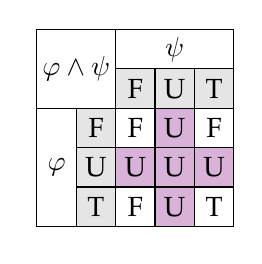
\begin{tikzpicture}[scale=.5]
\begin{scope}[violet!30]
\fill  (2,-1) rectangle (3,-4);
\fill  (1,-2) rectangle (4,-3);
\end{scope}
\node at (0,0){};
\draw [step=1cm] (-1,-4) node (v1) {} grid (4,1);
\draw[fill=white]  (v1) rectangle (0,-1);
\draw[fill=white]  (-1,1) rectangle (1,-1) node (v2) {};
\draw[fill=white]  (1,1) rectangle (4,0);
\draw[fill=black, opacity=.1]  (v2) node (v3) {} rectangle (4,0);
\draw[fill=black, opacity=.1]  (v3) rectangle (0,-4);
\node at (0,0) {$\varphi\land \psi$};
\node at (-0.5,-2.5) {$\varphi$};
\node at (2.5,0.5) {$\psi$};
% The gray area
%     gray row
\node at (0.5,-1.5) {F};
\node at (0.5,-2.5) {U};
\node at (0.5,-3.5) {T};
%     gray column
\node at (1.5,-0.5) {F};
\node at (2.5,-0.5) {U};
\node at (3.5,-0.5) {T};
%     the white grid
%     1st row
\node at (1.5,-1.5) {F};
\node at (2.5,-1.5) {U};
\node at (3.5,-1.5) {F};
%     2nd row
\node at (1.5,-2.5) {U};
\node at (2.5,-2.5) {U};
\node at (3.5,-2.5) {U};
%     3rd row
\node at (1.5,-3.5) {F};
\node at (2.5,-3.5) {U};
\node at (3.5,-3.5) {T};
\end{tikzpicture}
\; %%%%%%%%%%%%%%%%%%%%%%%%%%%%%%%%%% KÉT KÉP KÖZTI SZÜNET %%%%%%%%%%%%%%%%%%%%%%%%%%%%%%%%%%%%%%%%%%%5
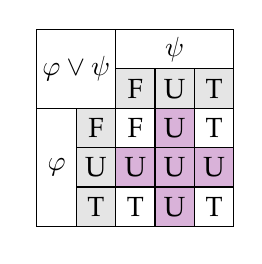
\begin{tikzpicture}[scale=.5]
\begin{scope}[violet!30]
\fill  (2,-1) rectangle (3,-4);
\fill  (1,-2) rectangle (4,-3);
\end{scope}
\node at (0,0){};
\draw [step=1cm] (-1,-4) node (v1) {} grid (4,1);
\draw[fill=white]  (v1) rectangle (0,-1);
\draw[fill=white]  (-1,1) rectangle (1,-1) node (v2) {};
\draw[fill=white]  (1,1) rectangle (4,0);
\draw[fill=black, opacity=.1]  (v2) node (v3) {} rectangle (4,0);
\draw[fill=black, opacity=.1]  (v3) rectangle (0,-4);
\node at (0,0) {$\varphi\lor \psi$};
\node at (-0.5,-2.5) {$\varphi$};
\node at (2.5,0.5) {$\psi$};
% The gray area
%     gray row
\node at (0.5,-1.5) {F};
\node at (0.5,-2.5) {U};
\node at (0.5,-3.5) {T};
%     gray column
\node at (1.5,-0.5) {F};
\node at (2.5,-0.5) {U};
\node at (3.5,-0.5) {T};
%     the white grid
%     1st row
\node at (1.5,-1.5) {F};
\node at (2.5,-1.5) {U};
\node at (3.5,-1.5) {T};
%     2nd row
\node at (1.5,-2.5) {U};
\node at (2.5,-2.5) {U};
\node at (3.5,-2.5) {U};
%     3rd row
\node at (1.5,-3.5) {T};
\node at (2.5,-3.5) {U};
\node at (3.5,-3.5) {T};
\end{tikzpicture}\]
\end{minipage}%
&\pause%%%%%%%%%%%%%%%%%% --- PAUSE --- %%%%%%%%%%%%%%%%%%
\begin{minipage}{5.2cm}
\[\textsc{Strong conjectives}\]
\[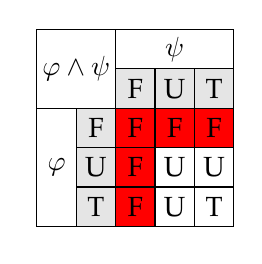
\begin{tikzpicture}[scale=.5]
\begin{scope}[red]
\fill  (2,-1) rectangle (1,-4);
\fill  (1,-2) rectangle (4,-1);
\end{scope}
\node at (0,0){};
\draw [step=1cm] (-1,-4) node (v1) {} grid (4,1);
\draw[fill=white]  (v1) rectangle (0,-1);
\draw[fill=white]  (-1,1) rectangle (1,-1) node (v2) {};
\draw[fill=white]  (1,1) rectangle (4,0);
\draw[fill=black, opacity=.1]  (v2) node (v3) {} rectangle (4,0);
\draw[fill=black, opacity=.1]  (v3) rectangle (0,-4);
\node at (0,0) {$\varphi\land \psi$};
\node at (-0.5,-2.5) {$\varphi$};
\node at (2.5,0.5) {$\psi$};
% The gray area
%     gray row
\node at (0.5,-1.5) {F};
\node at (0.5,-2.5) {U};
\node at (0.5,-3.5) {T};
%     gray column
\node at (1.5,-0.5) {F};
\node at (2.5,-0.5) {U};
\node at (3.5,-0.5) {T};
%     the white grid
%     1st row
\node at (1.5,-1.5) {F};
\node at (2.5,-1.5) {F};
\node at (3.5,-1.5) {F};
%     2nd row
\node at (1.5,-2.5) {F};
\node at (2.5,-2.5) {U};
\node at (3.5,-2.5) {U};
%     3rd row
\node at (1.5,-3.5) {F};
\node at (2.5,-3.5) {U};
\node at (3.5,-3.5) {T};
\end{tikzpicture}
\; %%%%%%%%%%%%%%%%%%%%%%%%%%%%%%%%%% KÉT KÉP KÖZTI SZÜNET %%%%%%%%%%%%%%%%%%%%%%%%%%%%%%%%%%%%%%%%%%%5
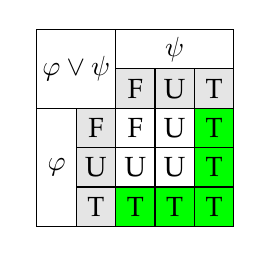
\begin{tikzpicture}[scale=.5]
\begin{scope}[green]
\fill  (4,-1) rectangle (3,-4);
\fill  (1,-4) rectangle (4,-3);
\end{scope}
\node at (0,0){};
\draw [step=1cm] (-1,-4) node (v1) {} grid (4,1);
\draw[fill=white]  (v1) rectangle (0,-1);
\draw[fill=white]  (-1,1) rectangle (1,-1) node (v2) {};
\draw[fill=white]  (1,1) rectangle (4,0);
\draw[fill=black, opacity=.1]  (v2) node (v3) {} rectangle (4,0);
\draw[fill=black, opacity=.1]  (v3) rectangle (0,-4);
\node at (0,0) {$\varphi\lor \psi$};
\node at (-0.5,-2.5) {$\varphi$};
\node at (2.5,0.5) {$\psi$};
% The gray area
%     gray row
\node at (0.5,-1.5) {F};
\node at (0.5,-2.5) {U};
\node at (0.5,-3.5) {T};
%     gray column
\node at (1.5,-0.5) {F};
\node at (2.5,-0.5) {U};
\node at (3.5,-0.5) {T};
%     the white grid
%     1st row
\node at (1.5,-1.5) {F};
\node at (2.5,-1.5) {U};
\node at (3.5,-1.5) {T};
%     2nd row
\node at (1.5,-2.5) {U};
\node at (2.5,-2.5) {U};
\node at (3.5,-2.5) {T};
%     3rd row
\node at (1.5,-3.5) {T};
\node at (2.5,-3.5) {T};
\node at (3.5,-3.5) {T};
\end{tikzpicture}\]
\end{minipage}
\end{tabular}
%My personal opinion is that since we are talking about \emph{settledness}, whether a truth of a statement is \emph{settled} or not, the strong operators are more appealing. \\ \hfill (Ruzsa always chose the weaks, and according to A.~Máté, the weak is more common in partial semantics.)
\end{frame}

\begin{frame}
	\frametitle{Modelling the undefined -- Kleene's logic(s)}
	\framesubtitle{Variations for implication}
\footnotesize

\[
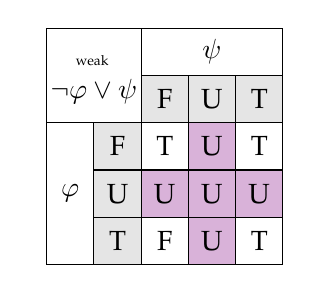
\begin{tikzpicture}[scale=.6]
\begin{scope}[violet!30]
\fill  (2,-1) rectangle (3,-4);
\fill  (1,-2) rectangle (4,-3);
\end{scope}
\node at (0,0){};
\draw [step=1cm] (-1,-4) node (v1) {} grid (4,1);
\draw[fill=white]  (v1) rectangle (0,-1);
\draw[fill=white]  (-1,1) rectangle (1,-1) node (v2) {};
\draw[fill=white]  (1,1) rectangle (4,0);
\draw[fill=black, opacity=.1]  (v2) node (v3) {} rectangle (4,0);
\draw[fill=black, opacity=.1]  (v3) rectangle (0,-4);
\node at (0,0) {$\begin{array}{c}\textup{\tiny weak }\\ \lnot \varphi\lor \psi \end{array}$};
\node at (-0.5,-2.5) {$\varphi$};
\node at (2.5,0.5) {$\psi$};
% The gray area
%     gray row
\node at (0.5,-1.5) {F};
\node at (0.5,-2.5) {U};
\node at (0.5,-3.5) {T};
%     gray column
\node at (1.5,-0.5) {F};
\node at (2.5,-0.5) {U};
\node at (3.5,-0.5) {T};
%     the white grid
%     1st row
\node at (1.5,-1.5) {T};
\node at (2.5,-1.5) {U};
\node at (3.5,-1.5) {T};
%     2nd row
\node at (1.5,-2.5) {U};
\node at (2.5,-2.5) {U};
\node at (3.5,-2.5) {U};
%     3rd row
\node at (1.5,-3.5) {F};
\node at (2.5,-3.5) {U};
\node at (3.5,-3.5) {T};
\end{tikzpicture}
\quad
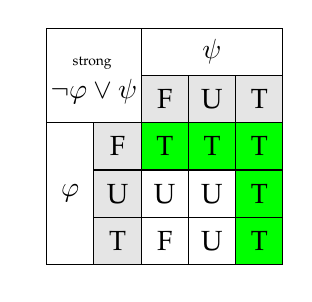
\begin{tikzpicture}[scale=.6]
%\fill[violet!30]  (2,-2) rectangle (3,-3);
\begin{scope}[green]
\fill  (4,-1) rectangle (3,-4);
\fill  (1,-1) rectangle (4,-2);
\end{scope}
\node at (0,0){};
\draw [step=1cm] (-1,-4) node (v1) {} grid (4,1);
\draw[fill=white]  (v1) rectangle (0,-1);
\draw[fill=white]  (-1,1) rectangle (1,-1) node (v2) {};
\draw[fill=white]  (1,1) rectangle (4,0);
\draw[fill=black, opacity=.1]  (v2) node (v3) {} rectangle (4,0);
\draw[fill=black, opacity=.1]  (v3) rectangle (0,-4);
\node at (0,0) {$\begin{array}{c}\textup{\tiny  strong }\\ \lnot \varphi\lor \psi \end{array}$};
\node at (-0.5,-2.5) {$\varphi$};
\node at (2.5,0.5) {$\psi$};
% The gray area
%     gray row
\node at (0.5,-1.5) {F};
\node at (0.5,-2.5) {U};
\node at (0.5,-3.5) {T};
%     gray column
\node at (1.5,-0.5) {F};
\node at (2.5,-0.5) {U};
\node at (3.5,-0.5) {T};
%     the white grid
%     1st row
\node at (1.5,-1.5) {T};
\node at (2.5,-1.5) {T};
\node at (3.5,-1.5) {T};
%     2nd row
\node at (1.5,-2.5) {U};
\node at (2.5,-2.5) {U};
\node at (3.5,-2.5) {T};
%     3rd row
\node at (1.5,-3.5) {F};
\node at (2.5,-3.5) {U};
\node at (3.5,-3.5) {T};
\end{tikzpicture}
\quad
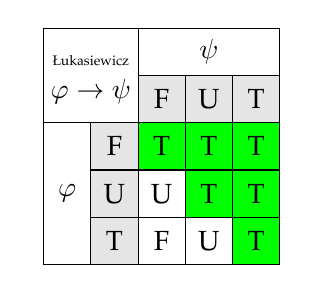
\begin{tikzpicture}[scale=.6]
\begin{scope}[green]
\fill  (4,-1) rectangle (3,-4);
\fill  (1,-1) rectangle (4,-2);
\fill  (3,-2) rectangle (2,-3);
\end{scope}
\node at (0,0){};
\draw [step=1cm] (-1,-4) node (v1) {} grid (4,1);
\draw[fill=white]  (v1) rectangle (0,-1);
\draw[fill=white]  (-1,1) rectangle (1,-1) node (v2) {};
\draw[fill=white]  (1,1) rectangle (4,0);
\draw[fill=black, opacity=.1]  (v2) node (v3) {} rectangle (4,0);
\draw[fill=black, opacity=.1]  (v3) rectangle (0,-4);
\node at (0,0) {$\begin{array}{c}\textup{\tiny {\L}ukasiewicz}\\ \varphi\to \psi \end{array}$};
\node at (-0.5,-2.5) {$\varphi$};
\node at (2.5,0.5) {$\psi$};
% The gray area
%     gray row
\node at (0.5,-1.5) {F};
\node at (0.5,-2.5) {U};
\node at (0.5,-3.5) {T};
%     gray column
\node at (1.5,-0.5) {F};
\node at (2.5,-0.5) {U};
\node at (3.5,-0.5) {T};
%     the white grid
%     1st row
\node at (1.5,-1.5) {T};
\node at (2.5,-1.5) {T};
\node at (3.5,-1.5) {T};
%     2nd row
\node at (1.5,-2.5) {U};
\node at (2.5,-2.5) {T};
\node at (3.5,-2.5) {T};
%     3rd row
\node at (1.5,-3.5) {F};
\node at (2.5,-3.5) {U};
\node at (3.5,-3.5) {T};
\end{tikzpicture}\]
\end{frame}


\begin{frame}
	\frametitle{About future}
%	\framesubtitle{classical connectives}
\begin{minipage}{.7\textwidth}
\[ \wintension[M]{w}{\FD \varphi} \defegy
\left\{ \begin{tomb}{ll}
   \mathrm T & \textup{ if } \forallp{h\ni w} \existsp {v>w} \; \wintension[M]{w}{\varphi}=\mathrm T
\\ \mathrm F & \textup{ if } \forallp{h\ni w} \existsp {v>w} \; \wintension[M]{w}{\varphi}=\mathrm F
\\ \mathrm U & \textup{ otherwise }
\end{tomb}\right. \]
\end{minipage}

\bigskip
\pause %%%%%%%%%%%%%%%%%%%%%%%% PAUSE %%%%%%%%%%%%%%%%%%%%%%%%%%%%%%%%%%%%%%
Now go back to the sea battle

\felirat{1.5}{1}{1}{4}{1}{
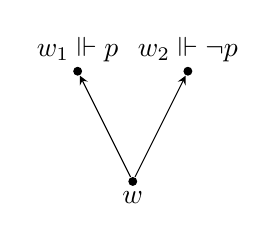
\begin{tikzpicture}[world/.style={inner sep=.4mm, fill=black, circle},>=stealth, scale=.7]
\node[world] (v1) at (0,-2) {};
\node[world] (v2) at (-1,0) {};
\node[world] (v3) at (1,0) {};
\node[anchor=south] at (v2) {$w_1\Vdash p$};
\node[anchor=south] at (v3) {$w_2\Vdash \lnot p$};
\node[anchor=north] at (v1) {$w$};
\draw[->]  (v1) edge (v2);
\draw[->]  (v1) edge (v3);
\end{tikzpicture}
}


\bigskip

%\dzsa{Problem}:

\[ \wintension{w}{\FD p} = \mathrm U, \qquad \wintension{w}{\FD \lnot p} = \mathrm U, \qquad \wintension{w}{\FD p \lor \FD \lnot p} = \mathrm U\]

%Why not $\wintension{w}{\FD p \lor \FD \lnot p} = \mathrm T$?

%\begin{center}
%\begin{minipage}{.9\textwidth}
%Prior pointed out that according to Aristotle \cemph{it is true already today}, that either there will or there will not be a sea-battle tomorrow
%\end{minipage}
%\end{center}
%\hfill P.~{\O}hrstr{\o}m, P.~Hasle 2011 (Stanford Enc.: Future Contingents)


\end{frame}

\end{document}
